%!TEX TS-program = pdflatex
\documentclass[preprint,showpacs,aps,prc,superscriptaddress]{revtex4-1}


% 论文基本配置,加载宏包等全局配置
% !TeX root = ./analysisnote.tex

% 载入所需的宏包
\usepackage{amsfonts}
\usepackage{amsmath}
\usepackage{txfonts}
\usepackage{amssymb}
\usepackage{mathrsfs}
\usepackage{graphicx}
\usepackage{dcolumn}
\usepackage{lineno}
\usepackage{hyperref}
\usepackage{multirow}
\usepackage{epstopdf}
\usepackage{natbib}
\usepackage{subfigure}
%\usepackage{tocloft}
%\setlength{\cftpartnumwidth}{3em}
%\def\l@section{\@dottedtocline{1}{2em}{2em}}
\renewcommand\thesection{\arabic{section}}
\renewcommand\thesubsection{\arabic{section}.\arabic{subsection}}
\renewcommand\thesubsubsection{\arabic{section}.\arabic{subsection}.\arabic{subsubsection}}
%arabic 阿拉伯数字 
%roman 小写的罗马数字 
%Roman 大写的罗马数字 
%alph 小写字母 
%Alph 大写字母
\hypersetup
{
    CJKbookmarks=true,
    bookmarksnumbered=true,
    bookmarksopen=true,
    breaklinks=true,
    colorlinks=true,
    linkcolor=blue,
    citecolor=blue,
    plainpages=false,
    pdfstartview=FitH
}
\newcommand{\snn}{\sqrt{s_\text{NN}}}
\newcommand{\pt}{p_T}
\newcommand{\gc}{GeV/$c$\ }
\newcommand{\bv}[1]{\textbf{\emph{{}#1}}}
\newcommand{\ffps}[1]{E_{{}#1}\frac{d^3\bv{N}_{{}#1}}{d\bv{p}^3_{{}#1}}}
\newcommand{\sfps}[1]{\frac{d^6\bv{N}_{{}#1}}{d\bv{r}^3_{{}#1}d\bv{p}^3_{{}#1}}}
\newcommand{\tfps}[1]{\frac{d^3\bv{N}_{{}#1}}{d\bv{p}^3_{{}#1}}}
\newcommand{\npart}{\langle N_{\textrm{part}}\rangle}

\begin{document}
%\preprint{}

\title{
\Huge{Analysis Note: \\ \textbf{Anti-flow of Kaon in Au+Au Collisions at $\sqrt{s_{NN}}$ = 3 - 3.9 GeV}}
}
\author{\Large{Zuowen Liu, Li-ke Liu, Xing Wu, Guoping Wang}}
%\affiliation{Key Laboratory of Quark $\&$ Lepton Physics (MOE) and Institute of Particle Physics, Central China Normal University, Wuhan, 430079, China}
%\date{\today \ \ \ Version 1.0}

% abstract
\begin{abstract}

\noindent\rule[0.25\baselineskip]{\textwidth}{1pt}
In this note, we present the measurement of anti-flow of kaons in Au+Au collisions at $\sqrt{s_{NN}}$ = 3.0, 3.2, 3.5, 3.9 GeV 
with the STAR experiment under its fixed target configuration at RHIC. 
Directed flow of $\pi^{\pm}$, $K^{\pm}$, $K_S^0$, p, and $\Lambda$ are presented in different centrality, transverse momentum, and rapidity intervals. 
$\pi^+$, $K^{\pm}$, and $K_S^0$ show anti-flow at low $p_T$ ($p_T <$ 0.6 GeV/c) at $\sqrt{s_{NN}}$ = 3.0, 3.2, 3.5, 3.9 GeV.
And the result have been compared with JAM model.
The data-model comparison indicates that anti-flow of kaons at low $p_T$ could be explained by shadowing effect from spectator.
\noindent\rule[0.25\baselineskip]{\textwidth}{1pt}

\end{abstract}


\newpage

\maketitle
%\listoffigures
%\listoftables
\tableofcontents
%\makeatletter
%\let\toc@pre\relax
%\let\toc@post\relax
%\makeatother

\clearpage

\newpage
% 正文部分
%\linenumbers
% !TeX root = ../analysisnote.tex

\section{Analysis setup}

\subsection{Dataset}

\blindtext

\subsection{Badrun rejection and centrality determination}

\blindtext

\subsection{Event and track selection}

\blindtext
% !TeX root = ../analysisnote.tex

\section{Analysis method}


\subsection{Event plane reconstruction}

\blindtext

\subsection{Particle identification}

\blindtext

\subsection{Efficiency correction}

\blindtext
\section{Results}

In this section, $v_1$ of $\pi$, K, p, $K^{0}_{S}$ and $\Lambda$ are presented as function of rapidity and transverse momentum at $\sqrt{s_{NN}}$ = 3.0, 3.2, 3.5, 3.9 GeV.
$\pi$, K, p $v_1$ were extracted based on event plane method, $K^{0}_{S}$ and $\Lambda$ $v_1$ were extracted by invariant mass method.
And the systematic uncertainty study was involved at the end of section.

\subsection{Directed flow of $\pi$, K, p}

\subsubsection{Rapidity dependence of $v_1$}

Fig.~\ref{fig:3p5gev_piKp_v1y} shows rapidity dependence of pions, kaons, and proton $v_1$ within 0-10\%, 10-40\%, 40-60\% centrality at $\sqrt{s_{NN}}$ = 3.5 GeV,
where the $p_T$ cut are $0.2 < p_T < 1.6~GeV/c$, $0.4 < p_T < 1.6~GeV/c$, $0.4 < p_T < 2.0~GeV/c$ for pions, kaons, and proton, respectively. 

\begin{figure}[hbt!]
\centering
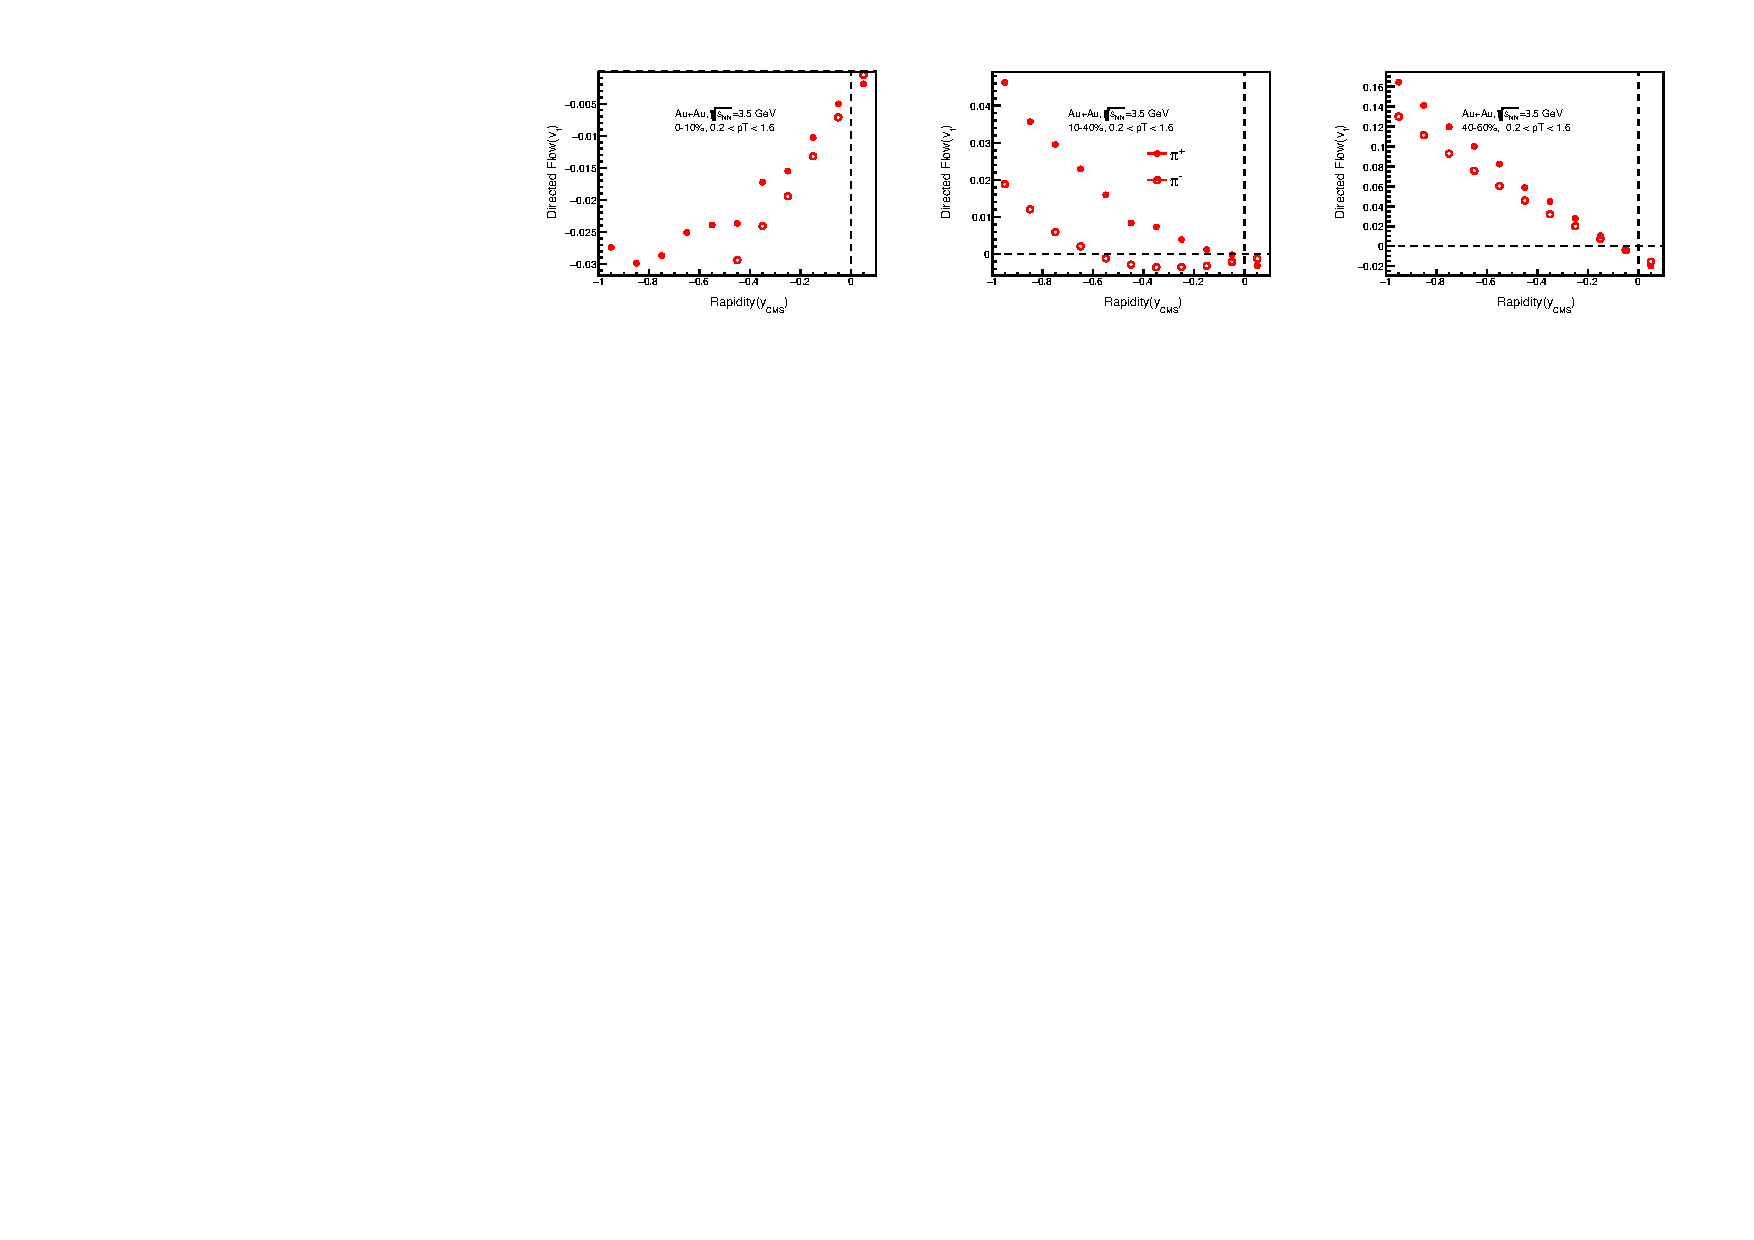
\includegraphics[width=0.85\linewidth]{figures/chapter03/3p5gev_pion_v1VSy.pdf}
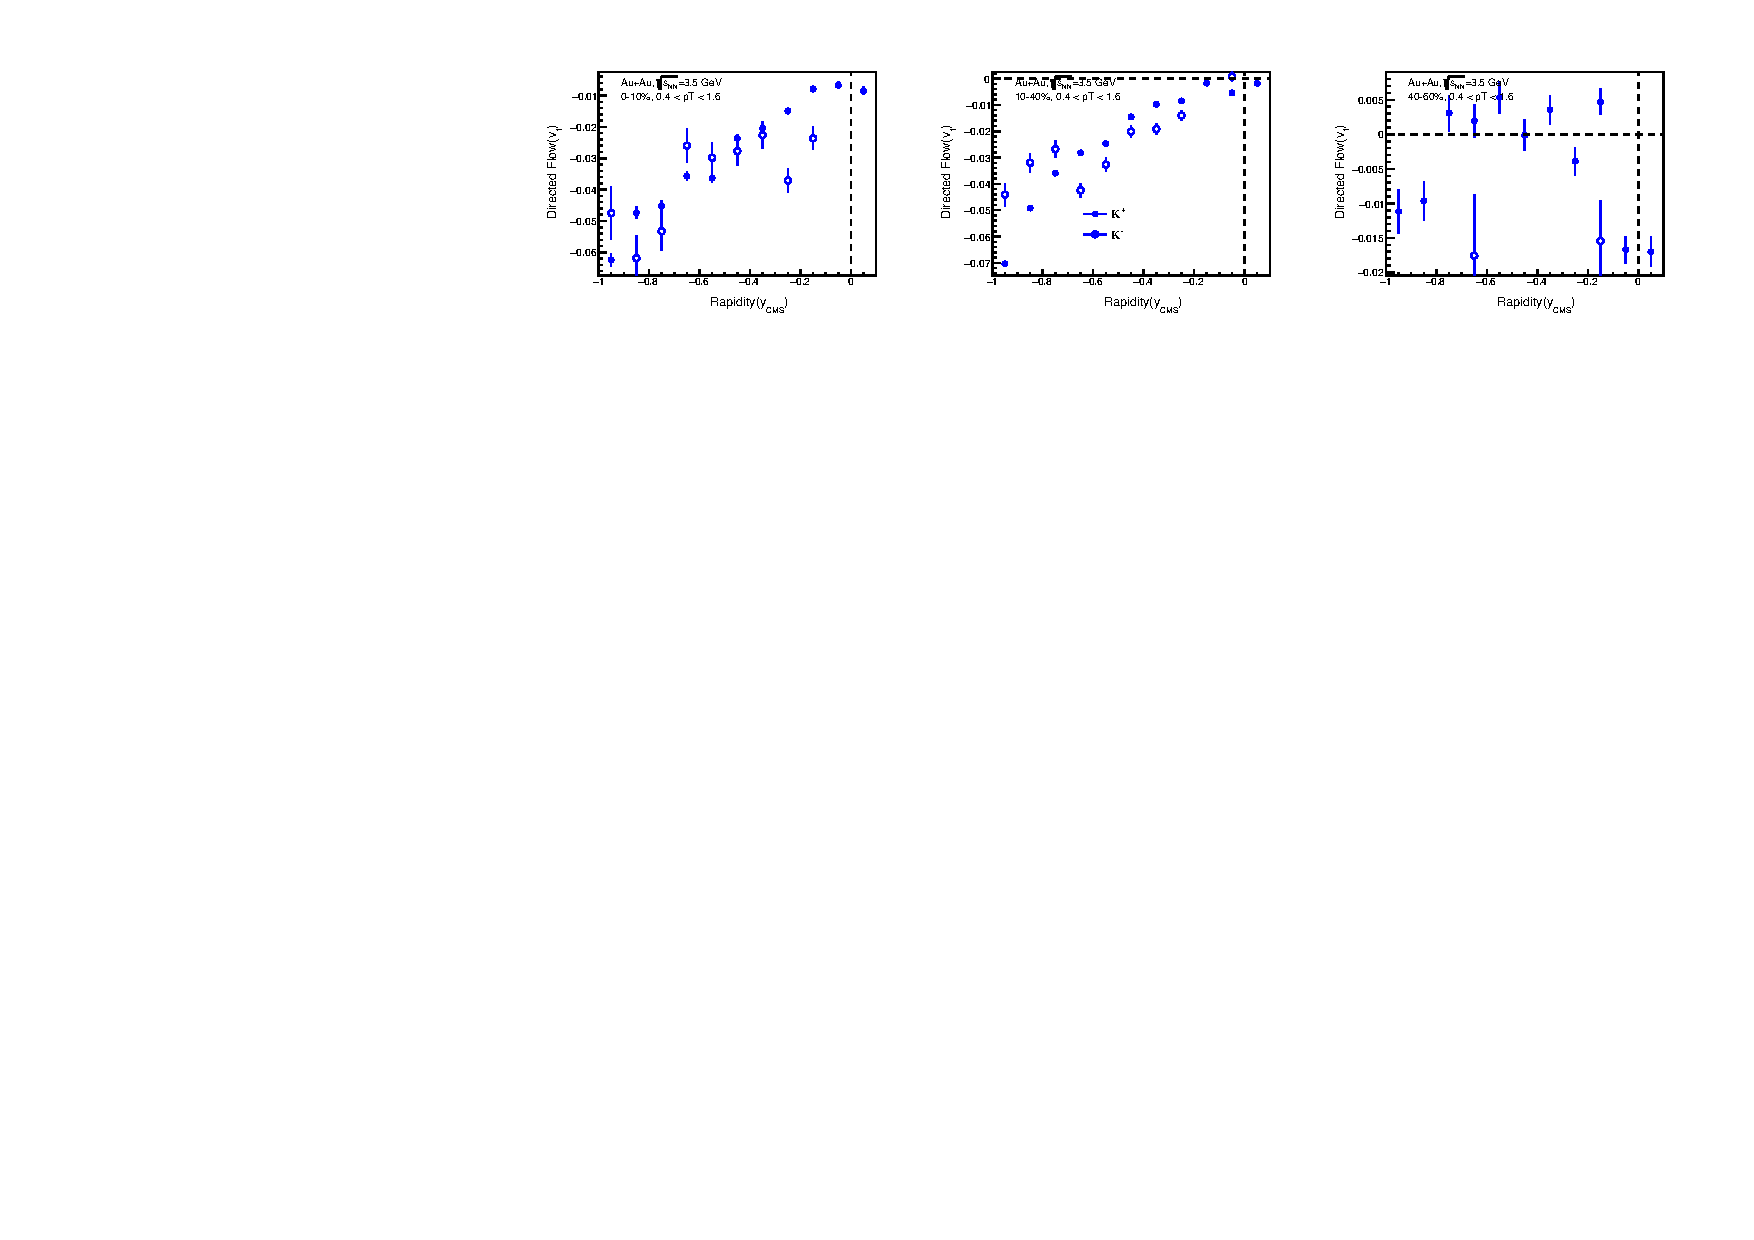
\includegraphics[width=0.85\linewidth]{figures/chapter03/3p5gev_kaon_v1VSy.pdf}
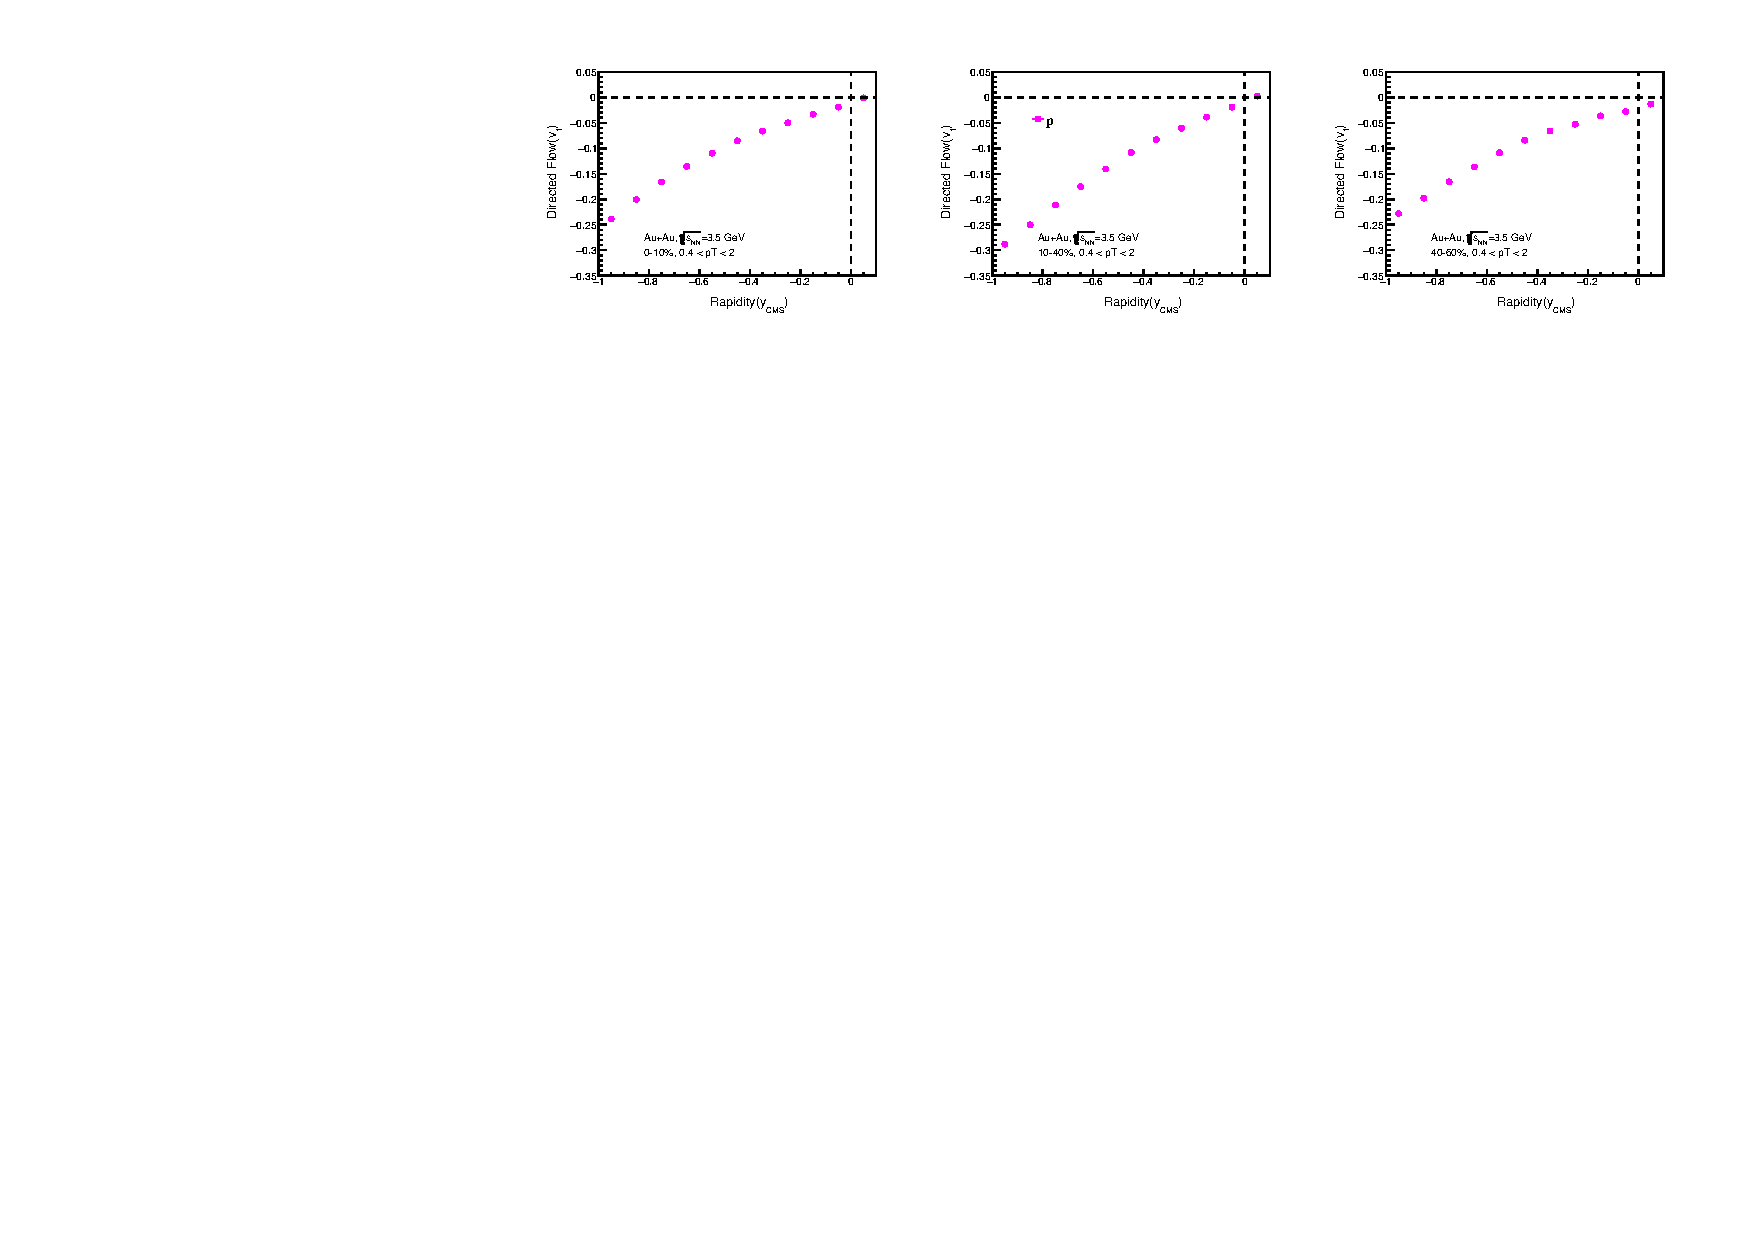
\includegraphics[width=0.85\linewidth]{figures/chapter03/3p5gev_proton_v1VSy.pdf}
\caption{$v_1$ of pions, kaons, and proton as function of rapidity at $\sqrt{s_{NN}}$ = 3.5 GeV.}
\label{fig:3p5gev_piKp_v1y}
\end{figure}

\subsubsection{Transverse momentum dependence of $v_1(y)$}

Fig.~\ref{fig:3p5gev_pion_v1y_pt_cent1} shows rapidity dependence of pion $v_1$ within $p_T$ windows in 10-40\% centrality at $\sqrt{s_{NN}}$ = 3.5 GeV.
And results in other centralities could be found in the appendix(0-10\%(Fig.~\ref{fig:3p5gev_pion_v1y_pt_cent2}), 40-60\%(Fig.~\ref{fig:3p5gev_pion_v1y_pt_cent0}))
Note that the solid and dashed line in the plots are cubic function: $v_1(y) = a*y + b*y^3$. 
The coefficient of the linear term "a" is so called $v_1$ slope in the mid-rapidity($dv_1/dy|_{y=0}$).

\begin{figure}[hbt!]
\centering
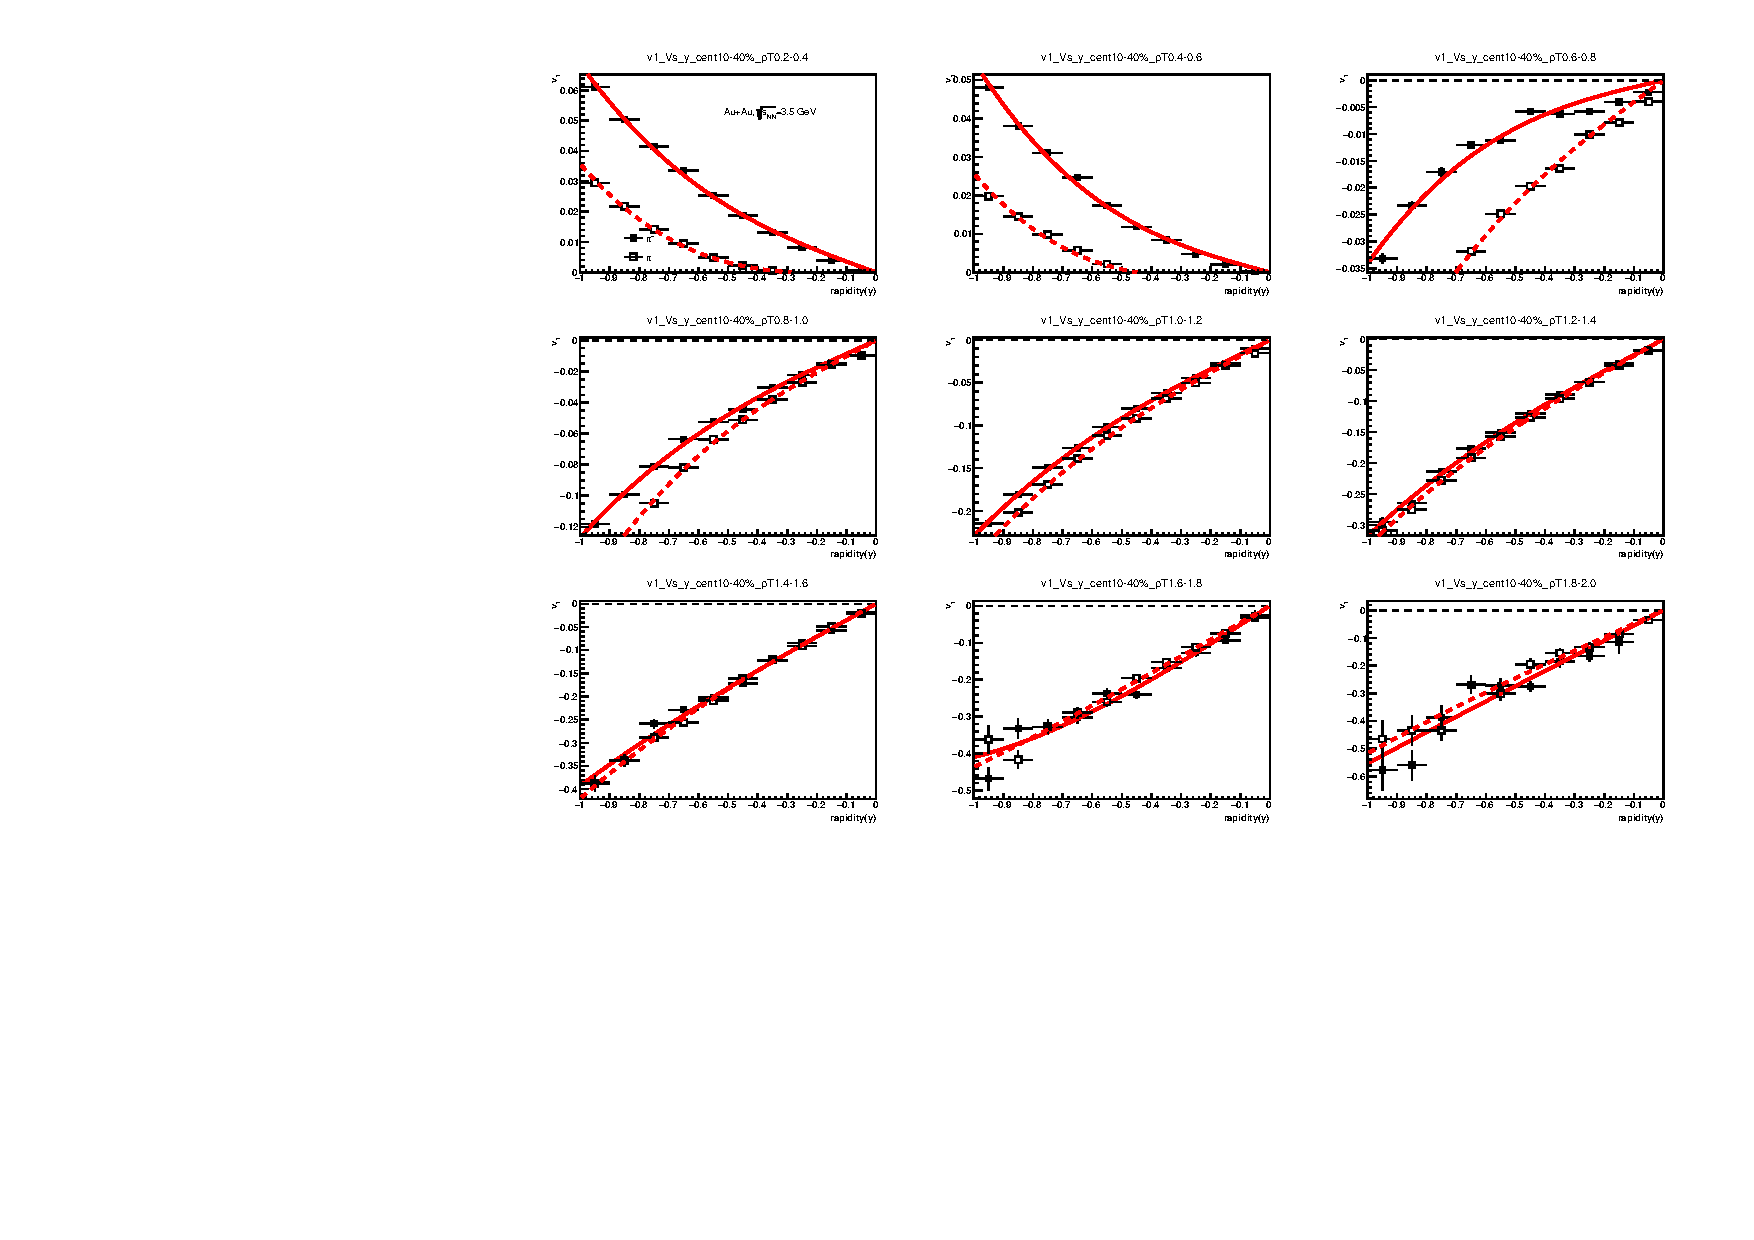
\includegraphics[width=0.85\linewidth]{figures/chapter03/3p5gev_pionp_v1VSy_9pT_cent1.pdf}
\caption{$v_1$ of pions as function of rapidity within $p_T$ windows in 10-40\% centrality at $\sqrt{s_{NN}}$ = 3.5 GeV.}
\label{fig:3p5gev_pion_v1y_pt_cent1}
\end{figure}

The $p_T$ dependence of $v_1$ slope is summarized in the Fig.~\ref{fig:3p5gev_pion_v1Slope_pt} for $\sqrt{s_{NN}}$ = 3.5 GeV.
Pion $v_1$ strength in the mid-rapidity show strong $p_T$ and centrality dependence, 
in the very-central collisions(0-10\%), there is no anti-flow(negative $v_1$ slope) at low $p_T$ for pions, 
while the slopes at low $p_T$ turn to negative in the mid-central and peripheral collisions.
In particular, the negative slopes are largest in magnitude in the peripheral collisions.
The centrality dependence of $v_1$ slope indicates that the pion anti-flow at low $p_T$ is due to 
shadowing effect from spectator.

\begin{figure}[hbt!]
\centering
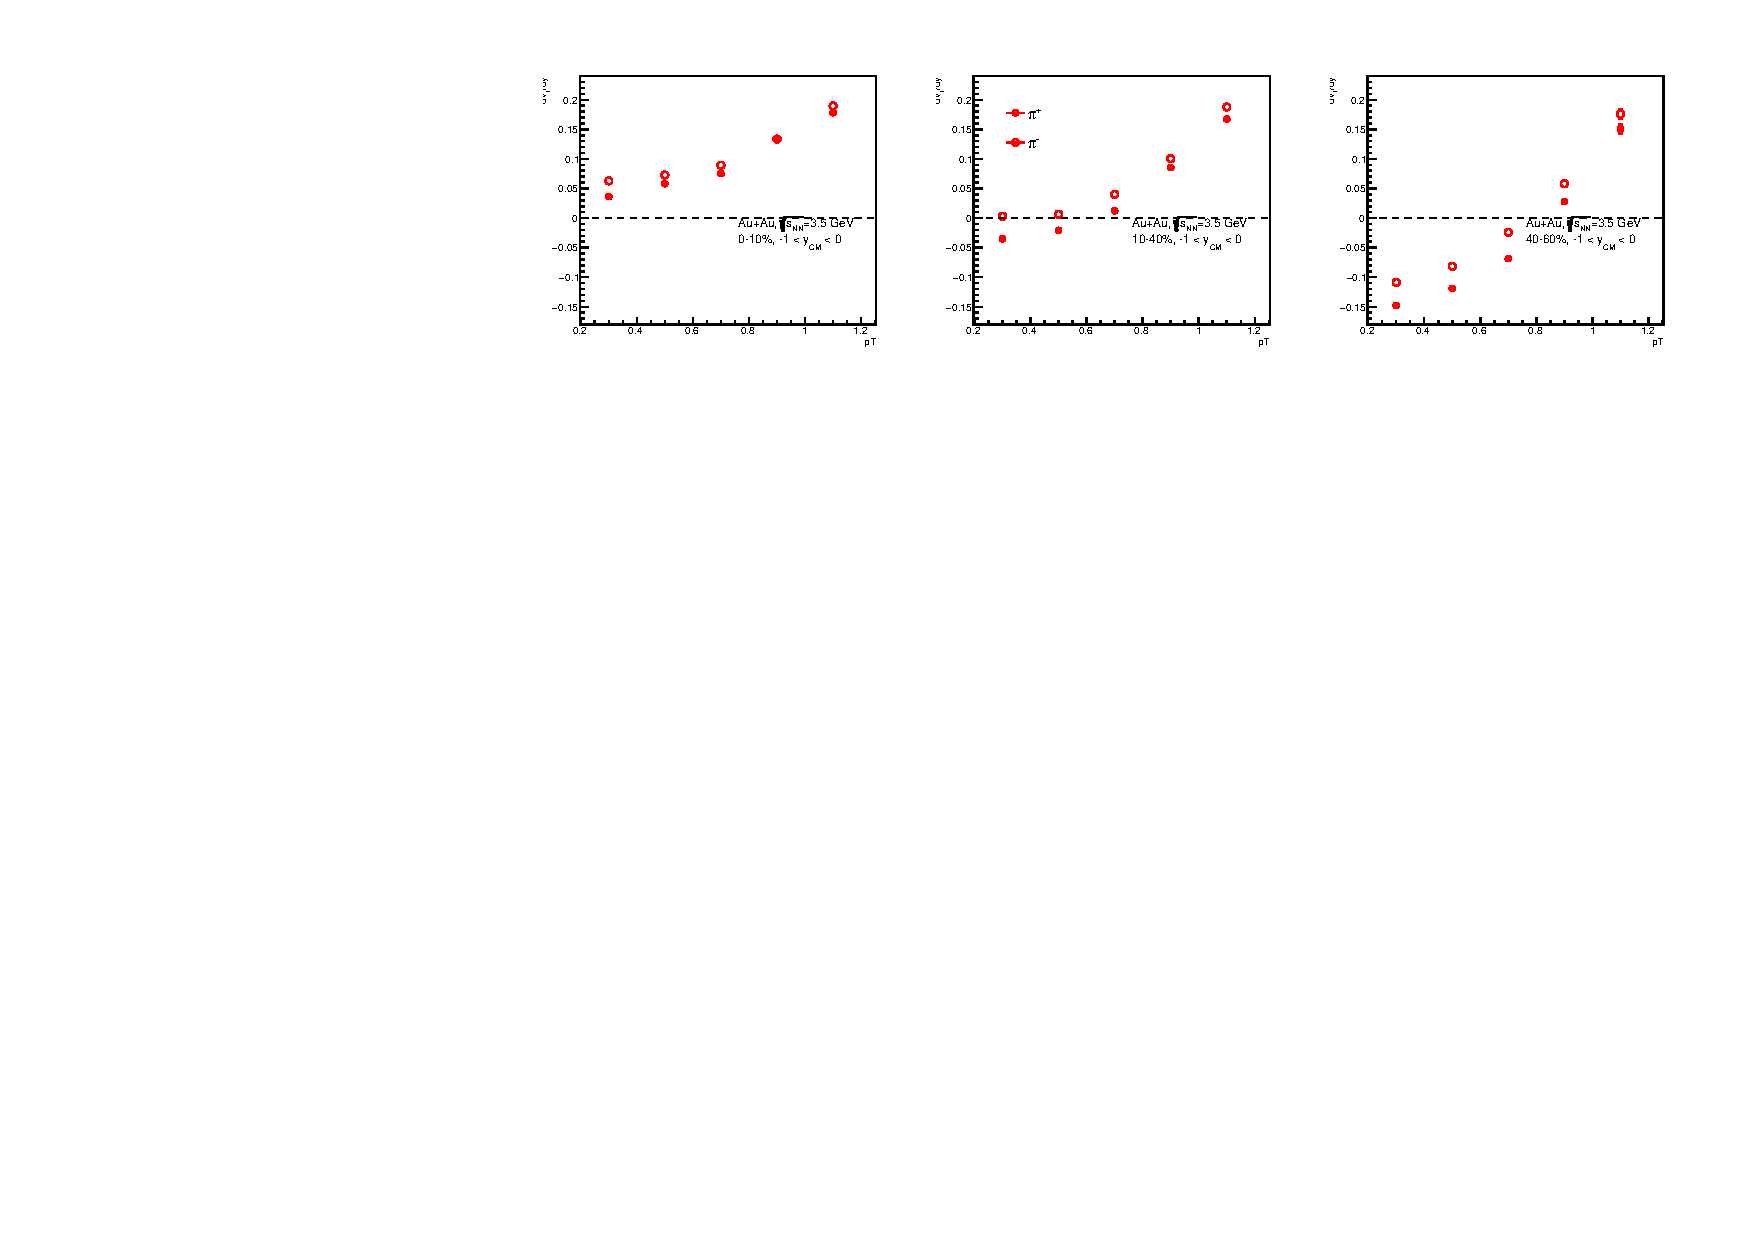
\includegraphics[width=0.95\linewidth]{figures/chapter03/3p5gev_pionp_v1Slope_pT.pdf}
\caption{$dv_1/dy|_{y=0}$ of pions as function of $p_T$ at $\sqrt{s_{NN}}$ = 3.5 GeV.}
\label{fig:3p5gev_pion_v1Slope_pt}
\end{figure}

Fig.~\ref{fig:3p5gev_kaon_v1Slope_pt} and Fig.~\ref{fig:3p5gev_proton_v1Slope_pt} show $p_T$ dependence of $v_1$ slope for kaons and proton, respectively.
The fitting plots could be found in the appendix.(Kaons:0-10\%(Fig.~\ref{fig:3p5gev_kaon_v1y_pt_cent2}), 10-40\%(Fig.~\ref{fig:3p5gev_kaon_v1y_pt_cent1}), 40-60\%(Fig.~\ref{fig:3p5gev_kaon_v1y_pt_cent0}). proton: 0-10\%(Fig.~\ref{fig:3p5gev_proton_v1y_pt_cent2}), 10-40\%(Fig.~\ref{fig:3p5gev_proton_v1y_pt_cent1}), 40-60\%(Fig.~\ref{fig:3p5gev_proton_v1y_pt_cent0})).
Kaons show anti-flow at low $p_T$ in the three centralities, 
while proton baryon didn't show anti-flow at low pT(positive slope in the three centralities).
The particle species dependence implies that the shadowing effect impact on the lighter meson and result in anti-flow at low $p_T$. 
The heavy baryon may go through the participant matter and remaining spectator without suffering strong shadowing effect as mesons.

For other energies, Fig.~\ref{fig:3gev_pion_v1Slope_pt}, Fig.~\ref{fig:3gev_kaon_v1Slope_pt}, and Fig.~\ref{fig:3gev_proton_v1Slope_pt} in the appendix show $p_T$ dependence of $v_1$ slope for pions, kaons, and proton at $\sqrt{s_{NN}}$ = 3.0 GeV, respectively.

\begin{figure}[hbt!]
\centering
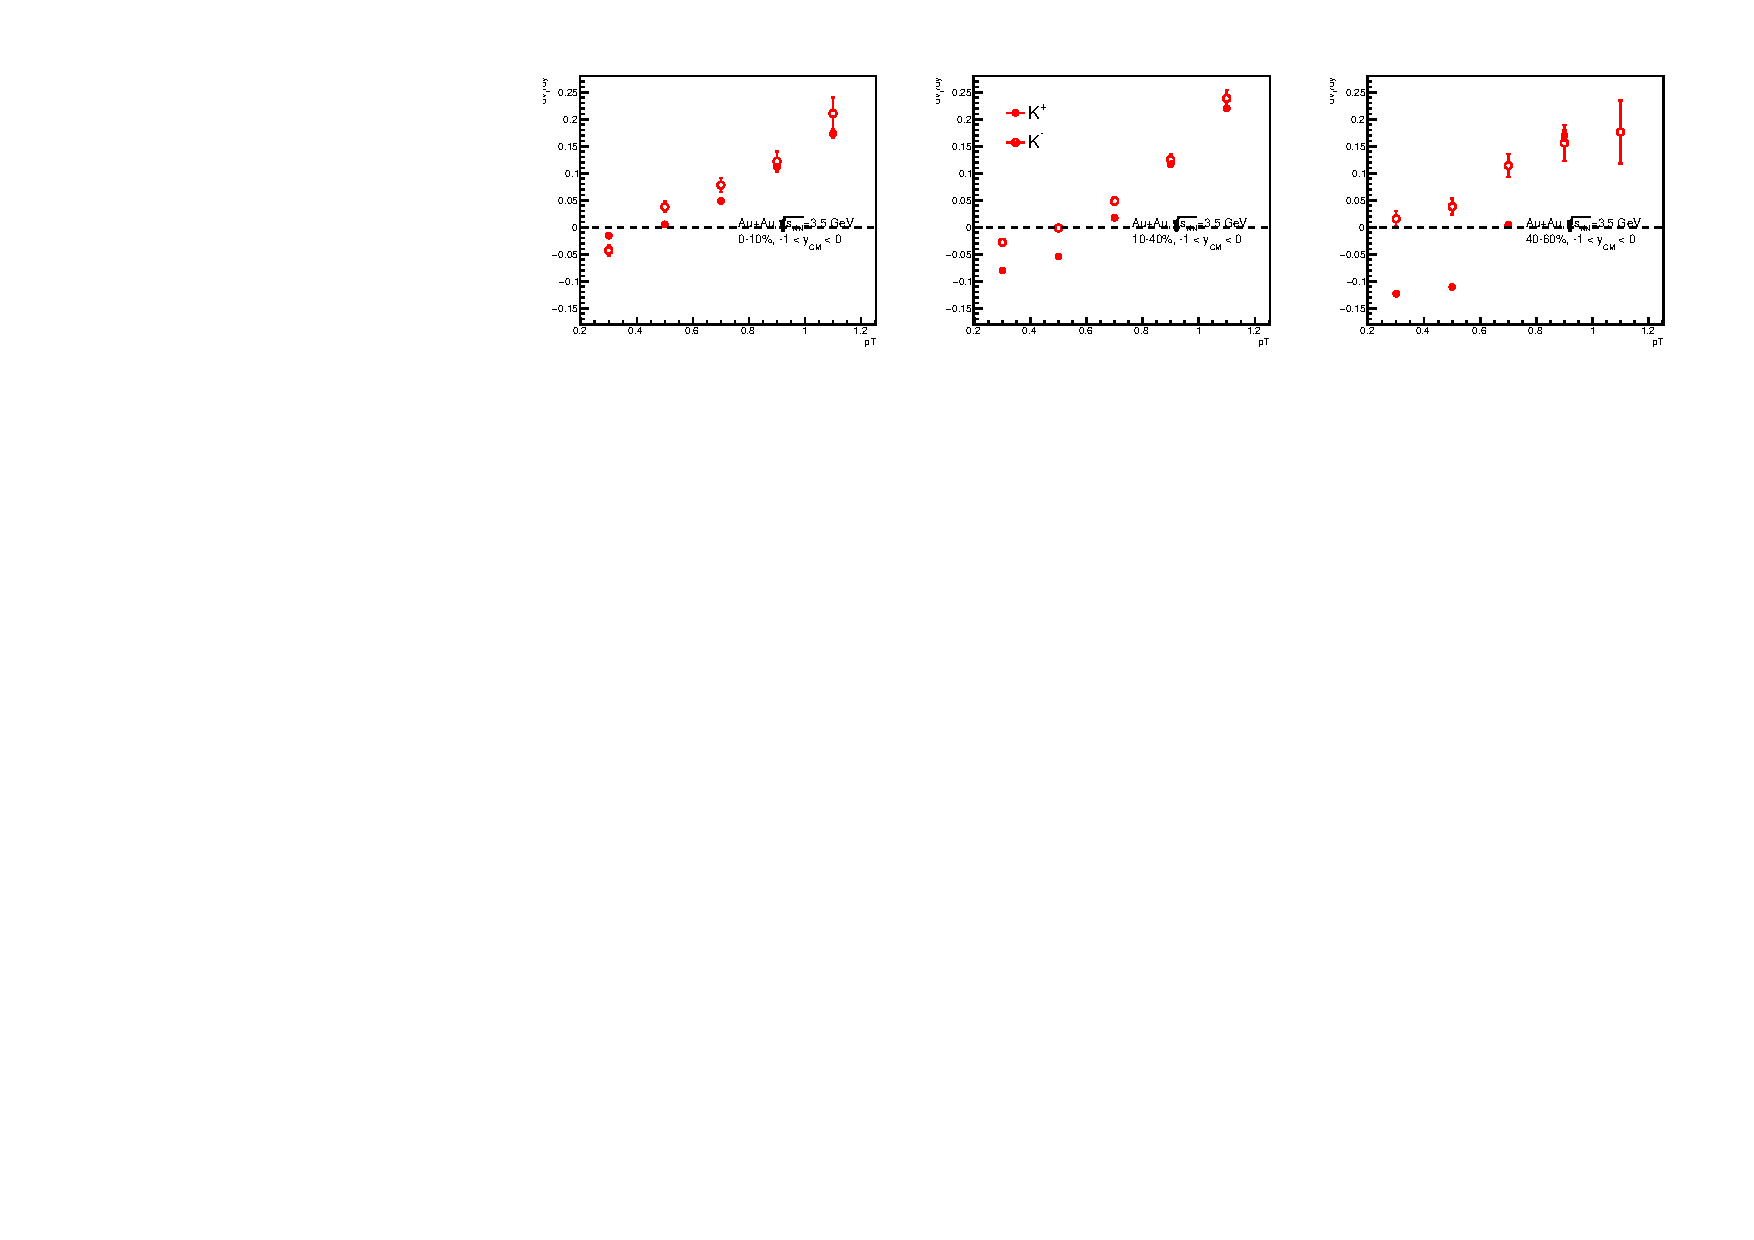
\includegraphics[width=0.95\linewidth]{figures/chapter03/3p5gev_kaonp_v1Slope_pT.pdf}
\caption{$dv_1/dy|_{y=0}$ of kaons as function of $p_T$ at $\sqrt{s_{NN}}$ = 3.5 GeV.}
\label{fig:3p5gev_kaon_v1Slope_pt}
\end{figure}

\begin{figure}[hbt!]
\centering
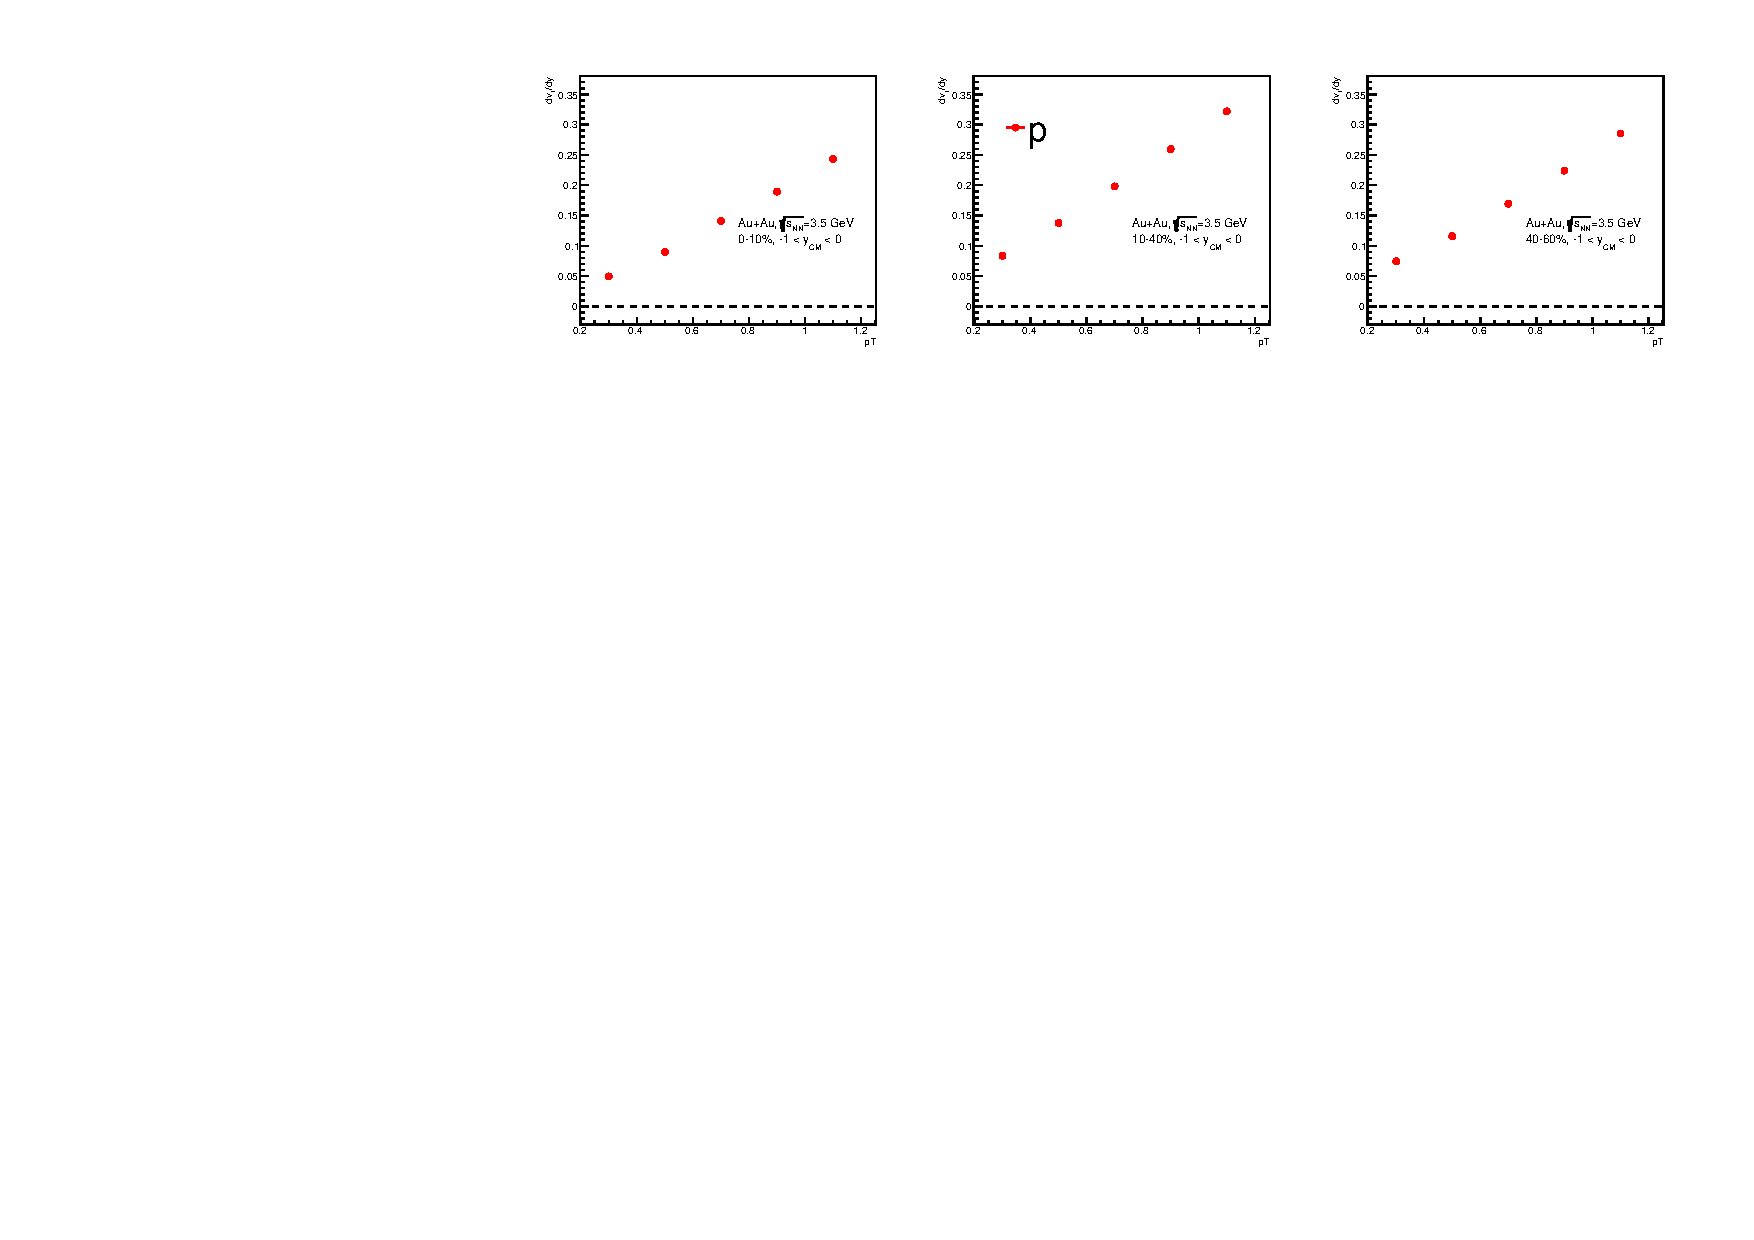
\includegraphics[width=0.95\linewidth]{figures/chapter03/3p5gev_protonp_v1Slope_pT.pdf}
\caption{$dv_1/dy|_{y=0}$ of proton as function of $p_T$ at $\sqrt{s_{NN}}$ = 3.5 GeV.}
\label{fig:3p5gev_proton_v1Slope_pt}
\end{figure}
    

\subsubsection{Systematic uncertainty}

The systematic uncertainty study could take random uncertainties into account~\cite{barlow2002systematic}, which are brought by detector effect, particle identification, and flow measurement method, etc.
In this analysis, we take track quality cuts (DCA and nHitsFit), PID cuts (n$\sigma_{particle}$ and $m^2$), and resolution as systematic uncertainty sources.
TABLE~\ref{tab:piKp_sysUnc} show the systematic uncertainty sources chosen for directed measurement of $\pi$, K, p.
We assume that these sources are uncorrelated. According to Barlow Test~\cite{barlow2002systematic}, the differences between the default source and the variation are required
to be smaller than the one of their statistical uncertainties, otherwise it would not be taken as systematic uncertainty since the statistical fluctuation dominants.
At last, the maximum deviation from the default value was chosen as the systematic uncertainty. 
The total systematic uncertainties could be obtained by the equation~\ref{eq:sysUnc_piKp}.

\begin{equation}
s y s. Unc_{\text {total }}=\sqrt{\left(y_{DCA}-y_{d e f}\right)^2+\left(y_{n H i tsFit}-y_{d e f}\right)^2+\left(y_{n \sigma}-y_{d e f}\right)^2+\left(y_{m^2}-y_{d e f}\right)^2+\left(y_{Res}-y_{d e f}\right)^2}
\label{eq:sysUnc_piKp}
\end{equation}

\begin{table}
    \centering
    \begin{tabular}{|c|c|c|c|} \hline  
         Cuts&  Default&  var1& var2\\ \hline  
         DCA($<$)&  3&  1& 2\\ \hline  
         nHitsFit($>$)&  15&  20& 25\\ \hline  
         n$\sigma_{particle} (<)$&  3&  2& 2.5\\ \hline  
         $m^2_\pi$&  [-0.1,0.15]&  [-0.05,0.1]
& \\ \hline 
 $m^2_K$& [0.16,0.36]
& [0.18,0.32]
&\\ \hline 
 $m^2_p$& [0.6, 1.2]& [0.7, 1.1]&\\ \hline 
         $R_{11}$&  EPD-C'&  EPD-D& \\ \hline 
    \end{tabular}
    \caption{Systematic uncertainty sources for $\pi$, K, p, Note that EPD-C' is EPD-AB vs. EPD-C' and TPC-B, and EPD-D is EPD-AB vs. EPD-D and TPC-B,
    which are shown in the Fig.~\ref{fig:1st_resolution}}
    \label{tab:piKp_sysUnc}
\end{table}

Fig.~\ref{fig:3p5gev_pion_v1y_sysUnc} illustrates the rapidity dependence of $v_1$ for pions from various systematic sources at  $\sqrt{s_{NN}}$ = 3.5 GeV.
$v_1$ of pions in the mid-central collisions are shown by Fig.~\ref{fig:3p5gev_pion_v1y}, where the bands stand for the systematic errors.
And Fig.~\ref{fig:3p5gev_pionplus_v1yPt_sysUnc} show $v_1(y)$ of $\pi^{+}$ within narrow $p_T$ windows, 
the $v_1$ slopes extracted in the mid-rapidity are summarized with Fig.~\ref{fig:3p5gev_pion_v1slopeIndex_sysUnc}.
At last, Fig.~\ref{fig:3p5gev_pion_v1slopePt} illustrates $p_T$ dependence of $v_1$ slope for pions, 
where $\pi^+$ shows anti-flow at low $p_T$, $\pi^-$ shows positive slopes. It might be explained by Columb effect. 
For other particles(kaons and proton) and other energies, the similary plots could be found in the appendix. 
\begin{figure}[hbt!]
\centering
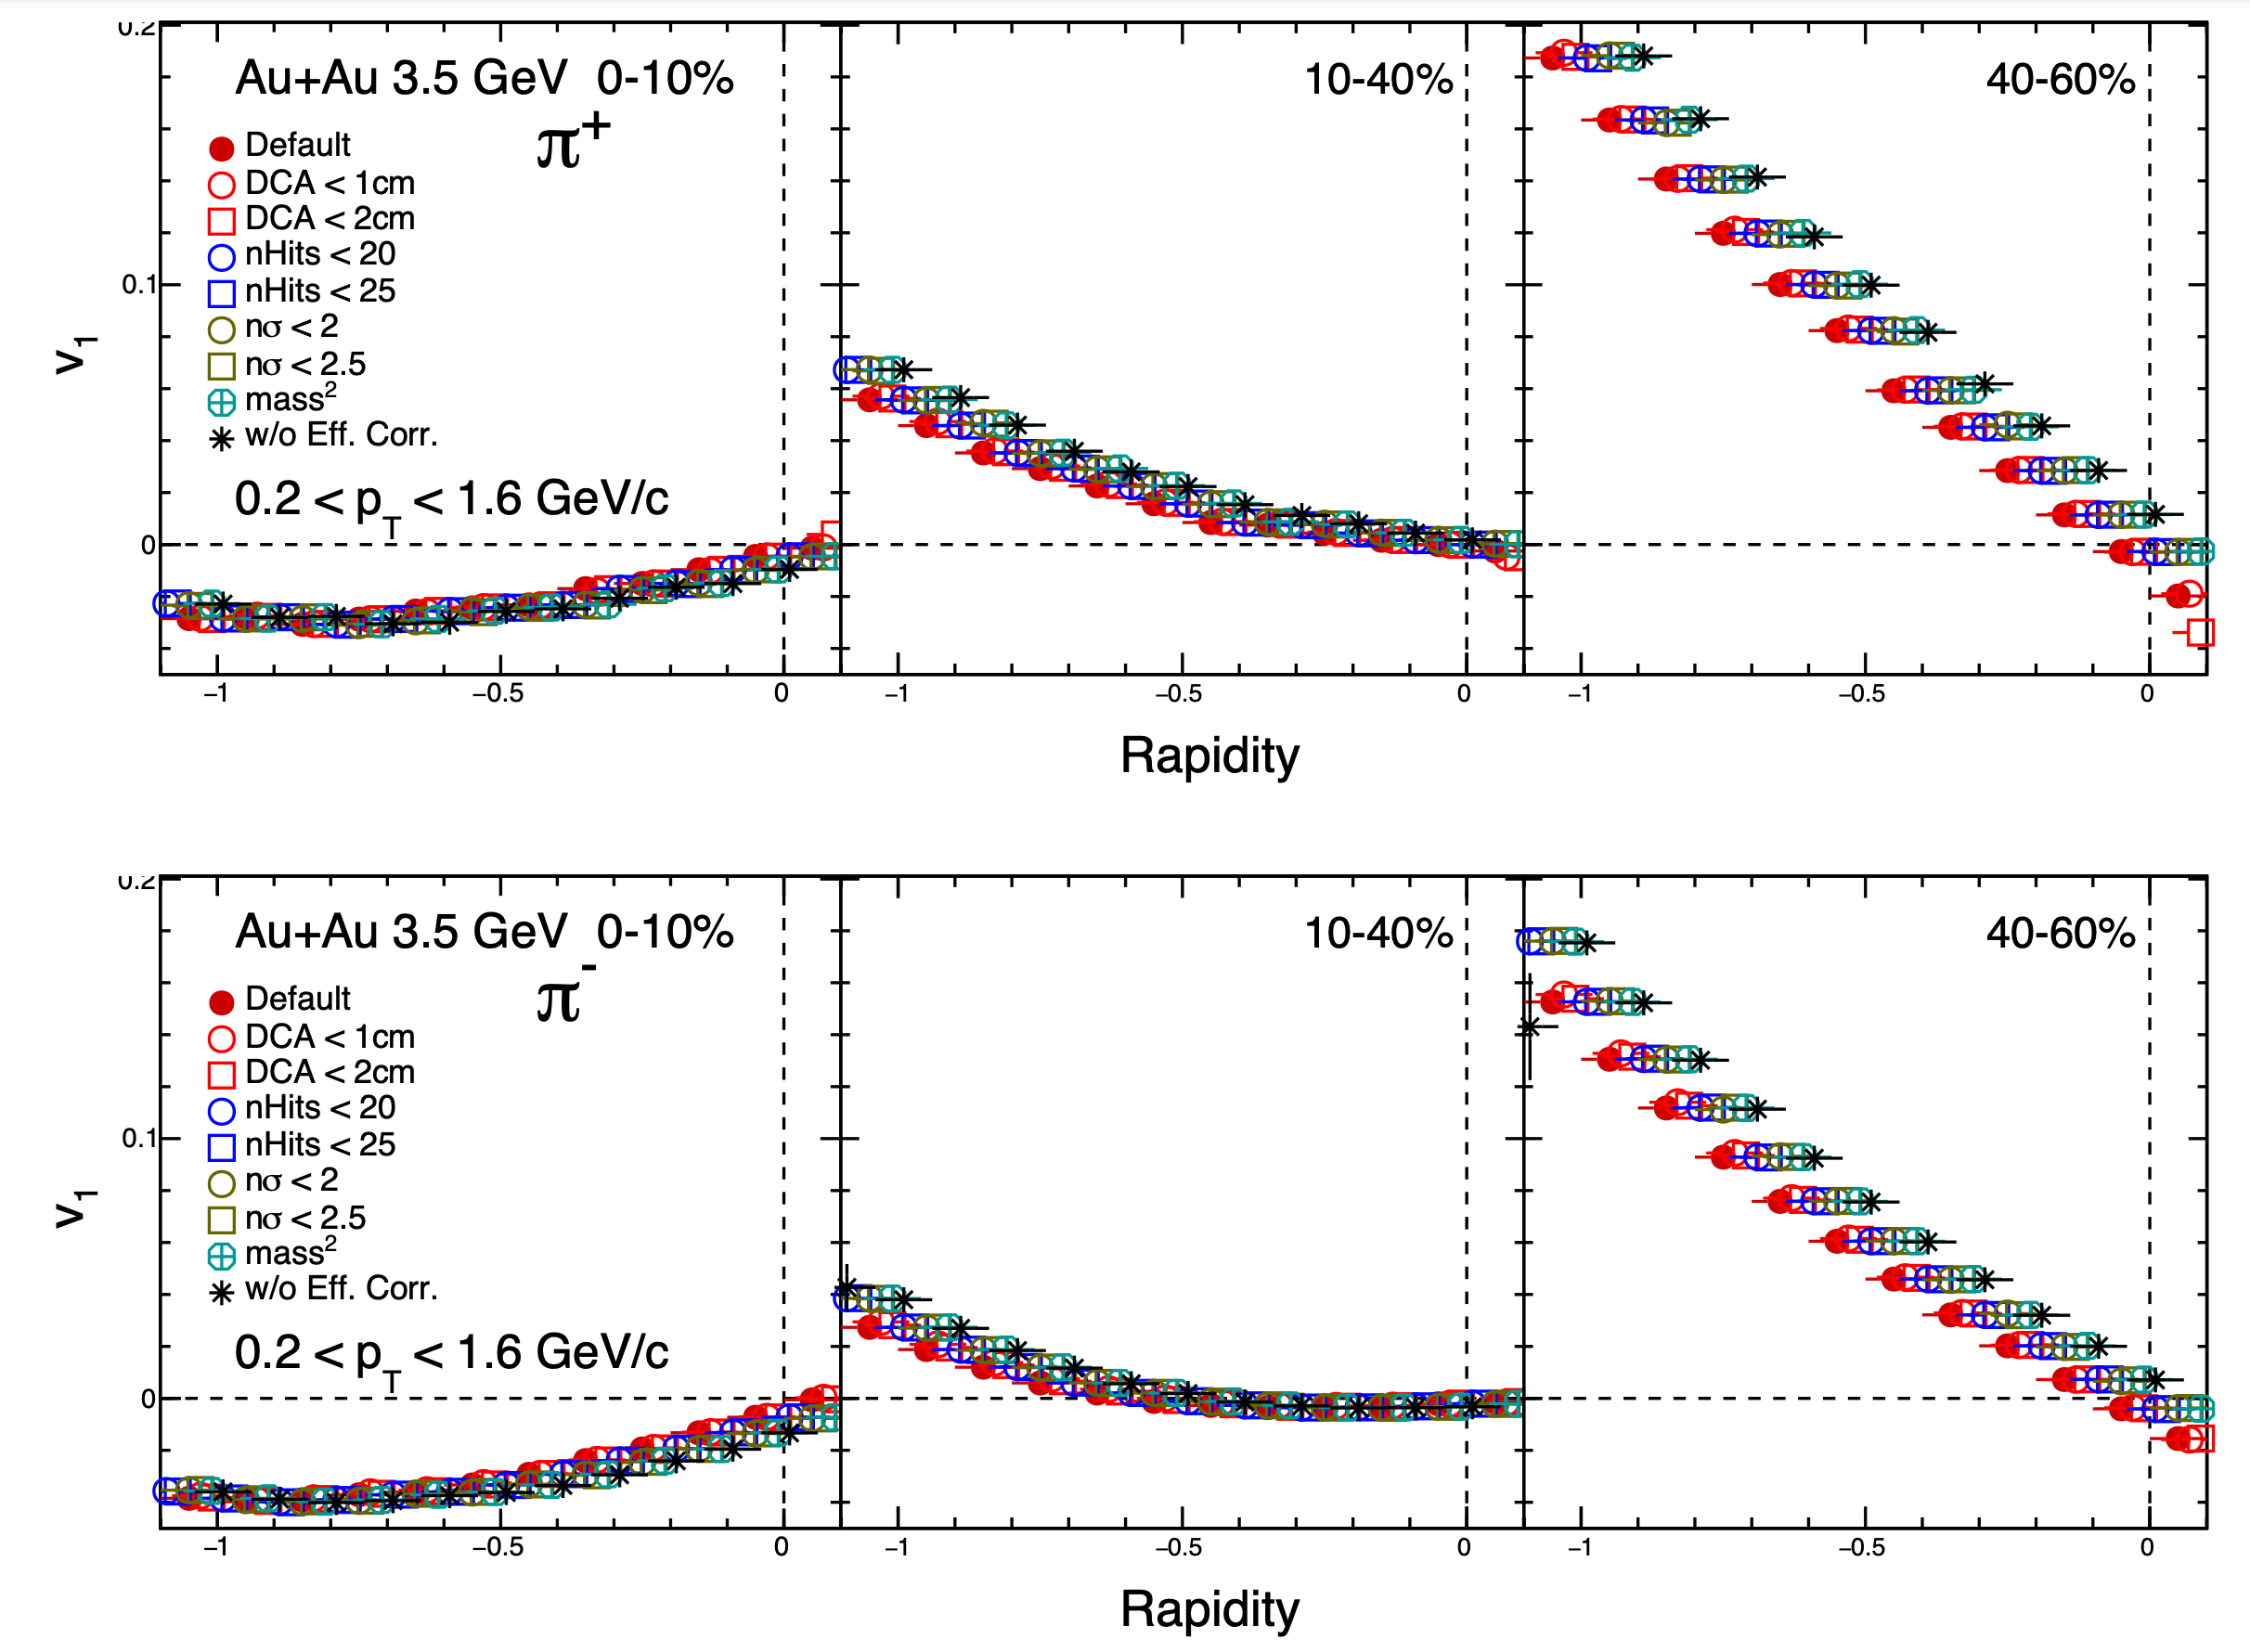
\includegraphics[width=0.95\linewidth]{figures/chapter03/3p5gev_pion_v1y_sysUnc.png}
\caption{$v_1$ of pions as function of rapidity from systematic sources at $\sqrt{s_{NN}}$ = 3.5 GeV.}
\label{fig:3p5gev_pion_v1y_sysUnc}
\end{figure}

\begin{figure}[hbt!]
\centering
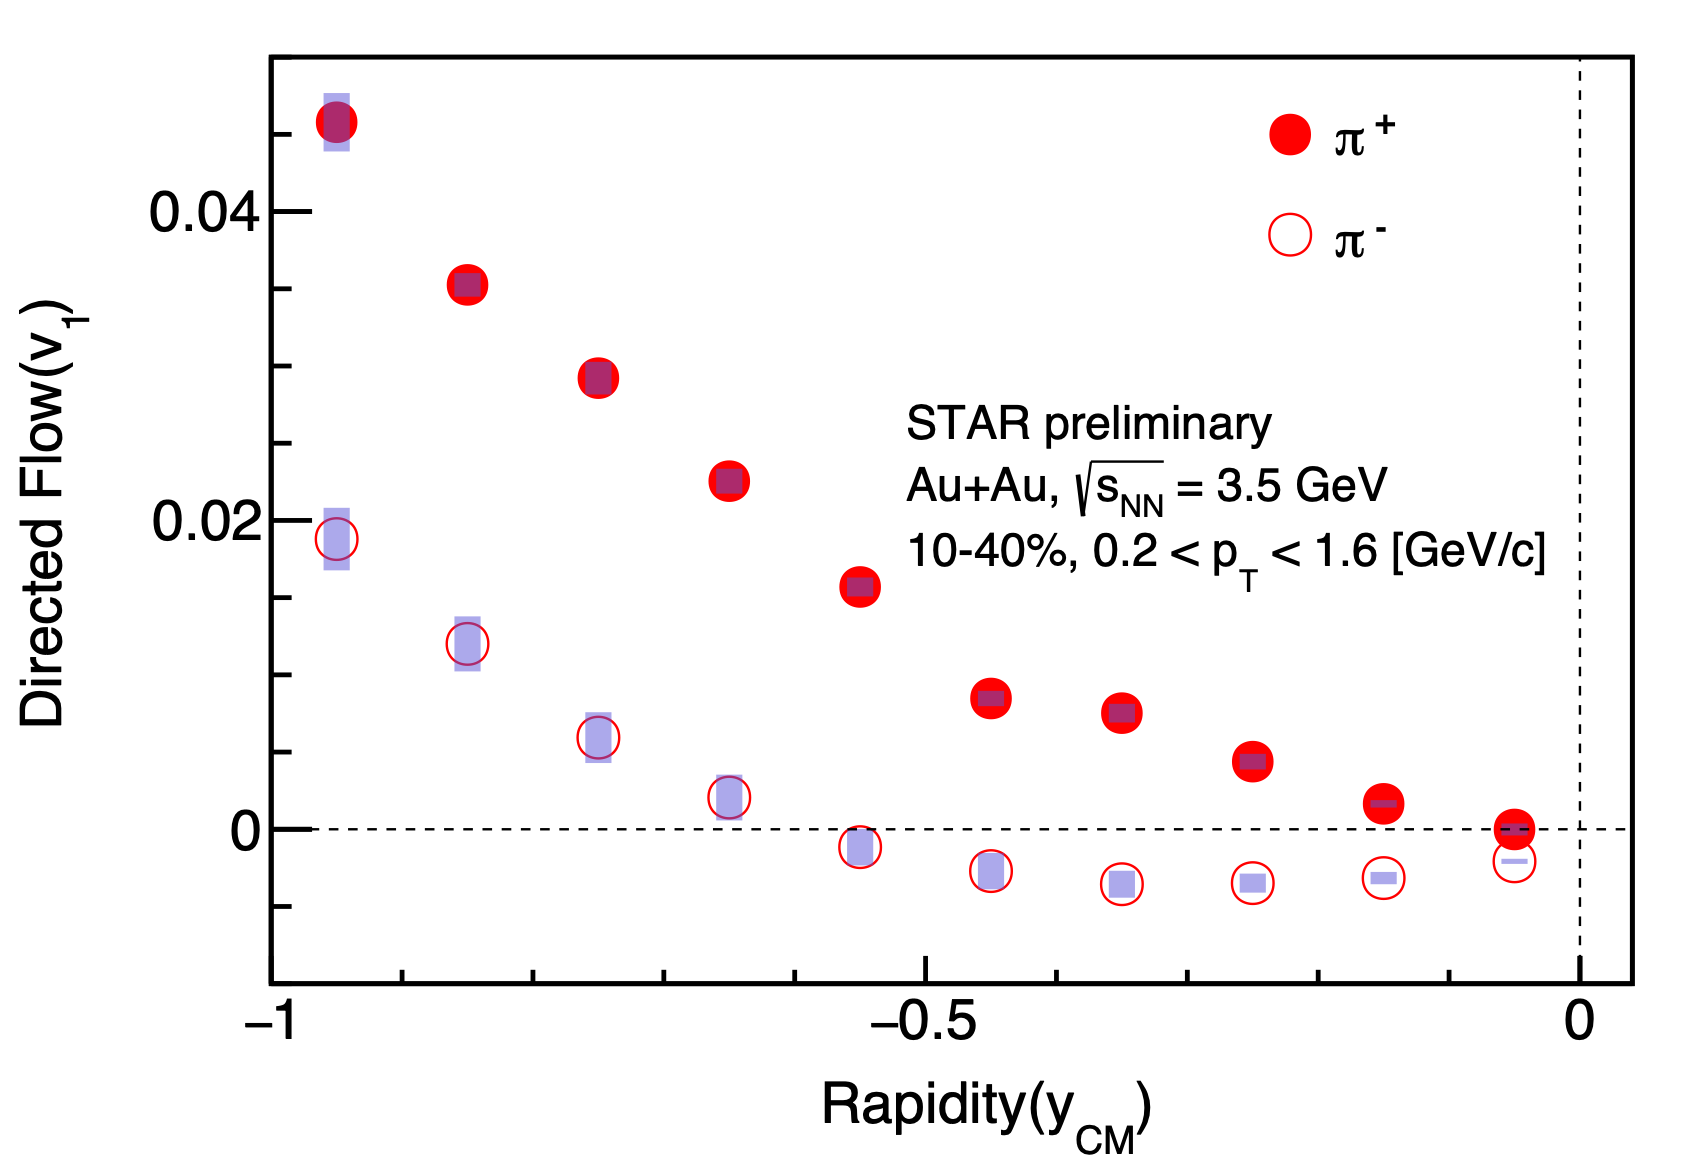
\includegraphics[width=0.65\linewidth]{figures/chapter03/3p5gev_pion_v1y.png}
\caption{$v_1$ of pions as function of rapidity at $\sqrt{s_{NN}}$ = 3.5 GeV.}
\label{fig:3p5gev_pion_v1y}
\end{figure}

\begin{figure}[hbt!]
\centering
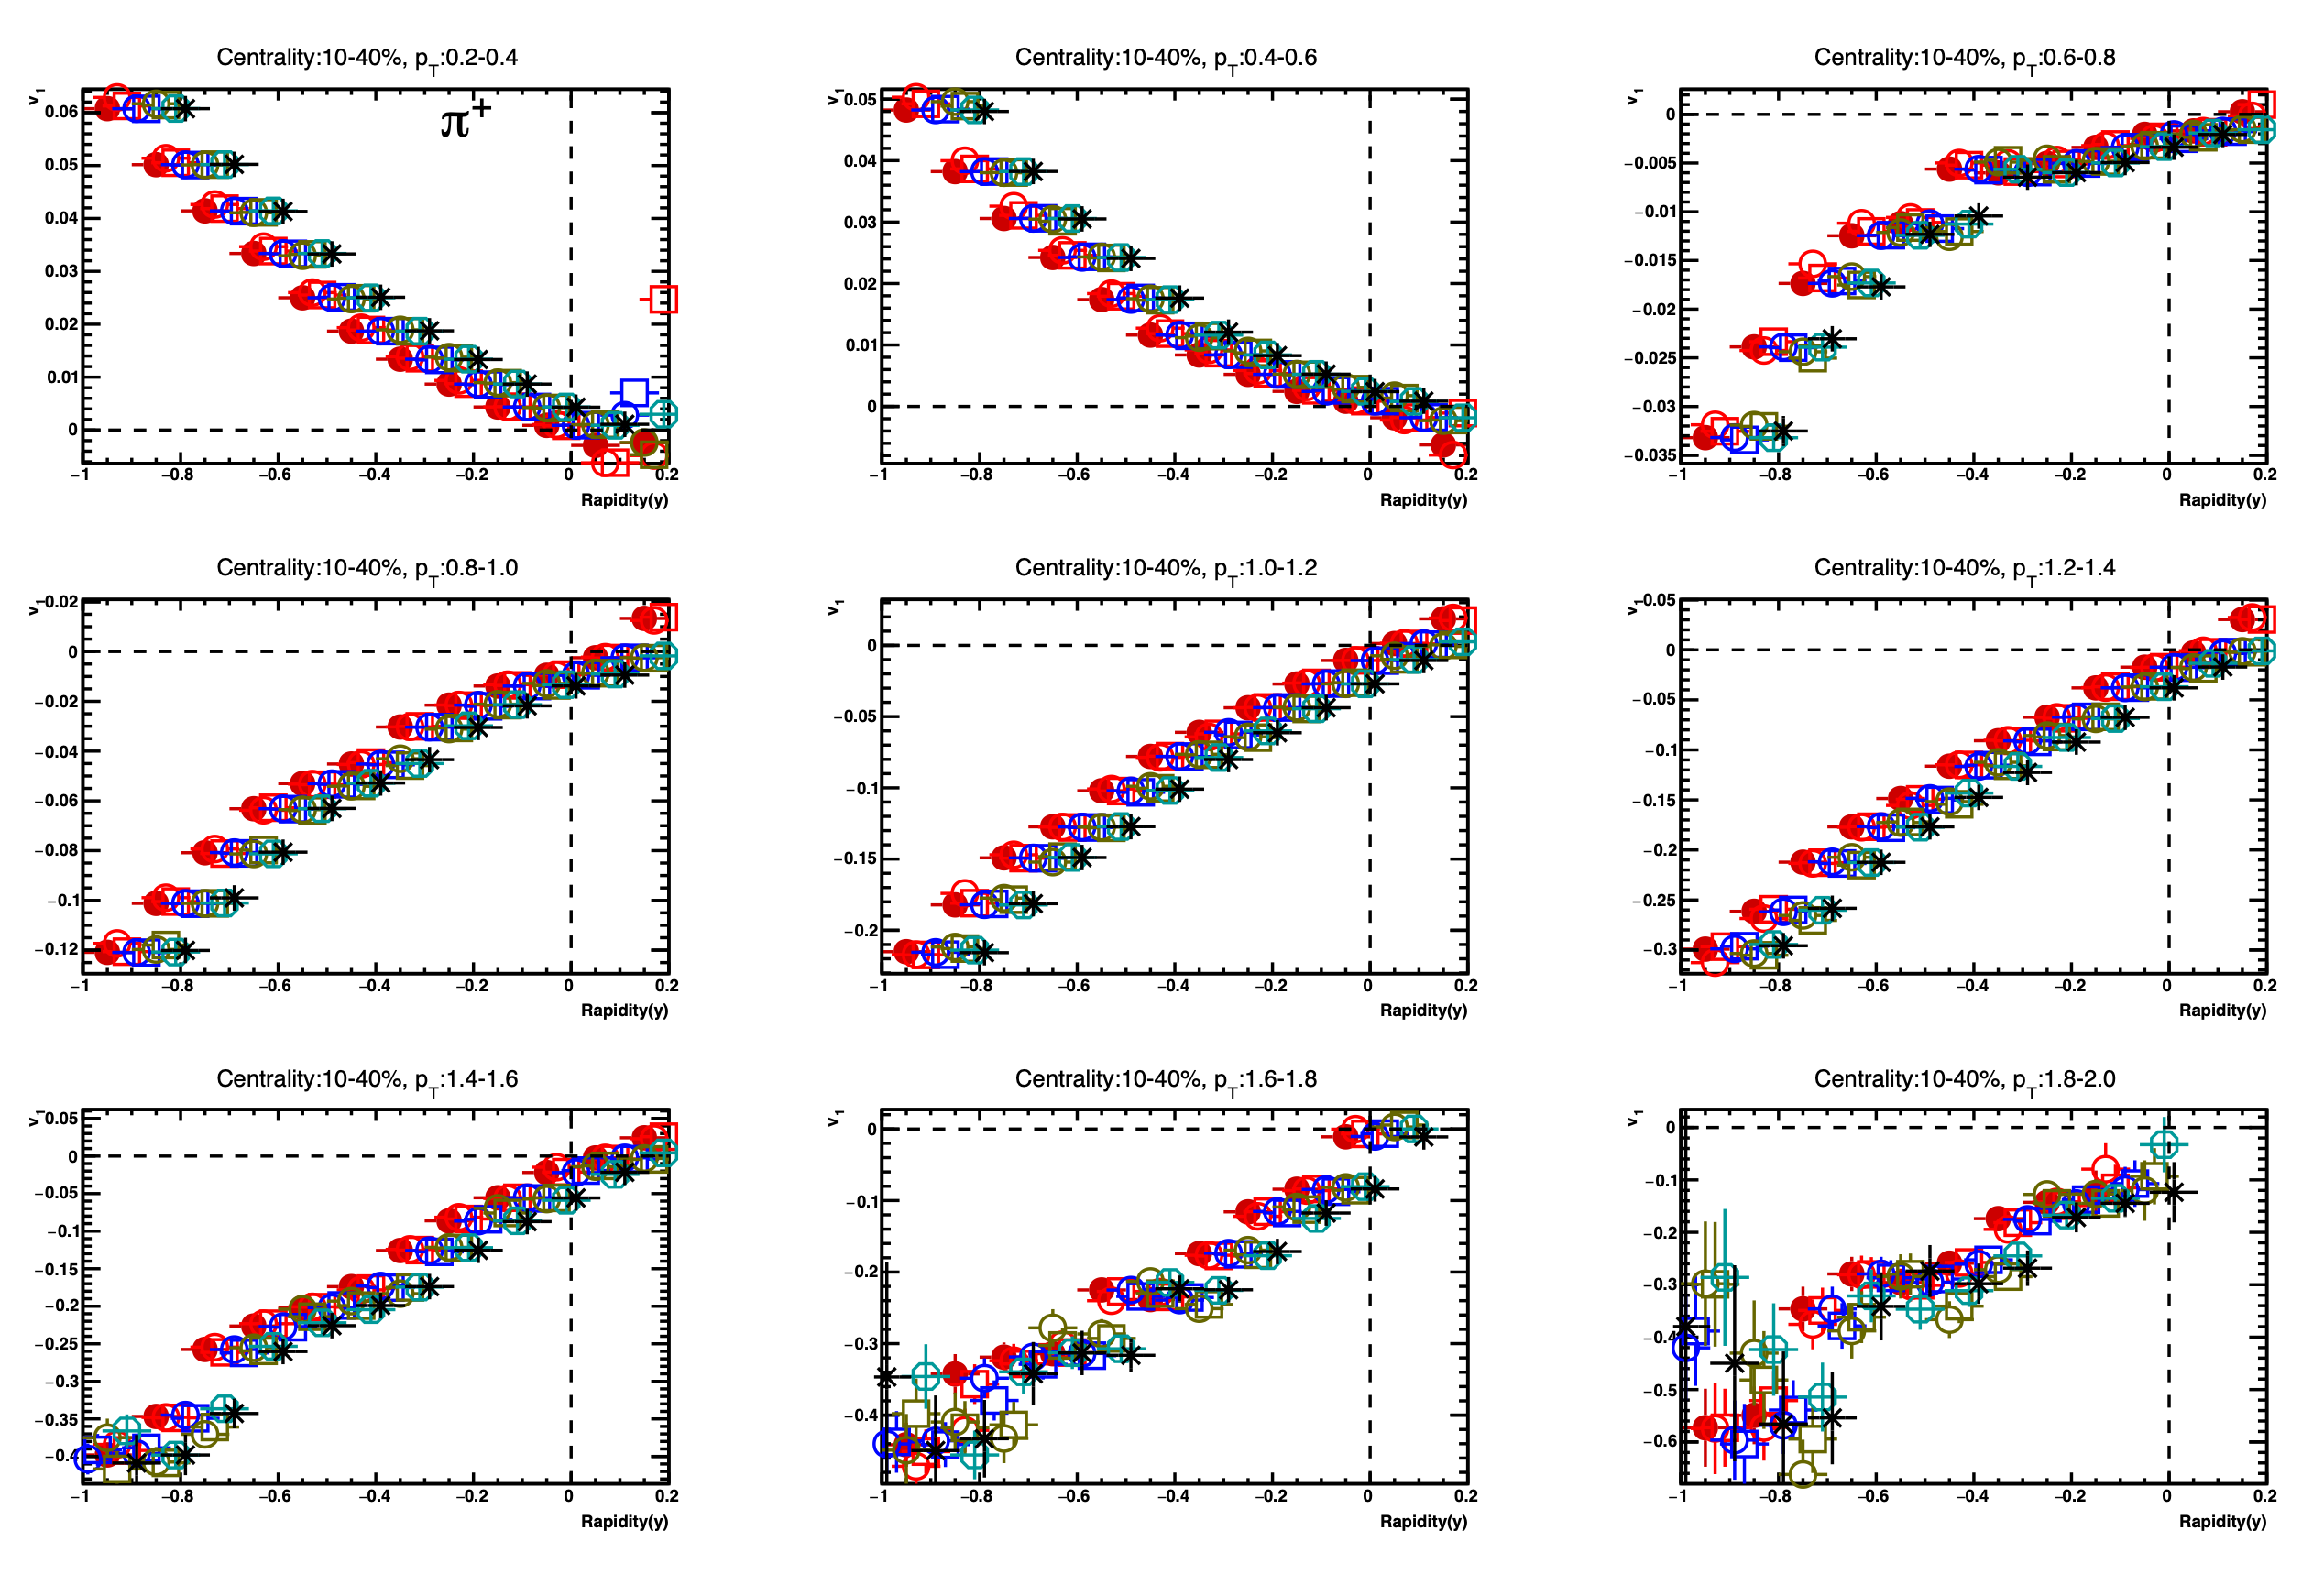
\includegraphics[width=0.95\linewidth]{figures/chapter03/3p5gev_pionplus_v1yPt_sysUnc.png}
\caption{$v_1$ of $\pi^+$ as function of rapidity within $p_T$ windows at $\sqrt{s_{NN}}$ = 3.5 GeV.}
\label{fig:3p5gev_pionplus_v1yPt_sysUnc}
\end{figure}

\begin{figure}[hbt!]
\centering
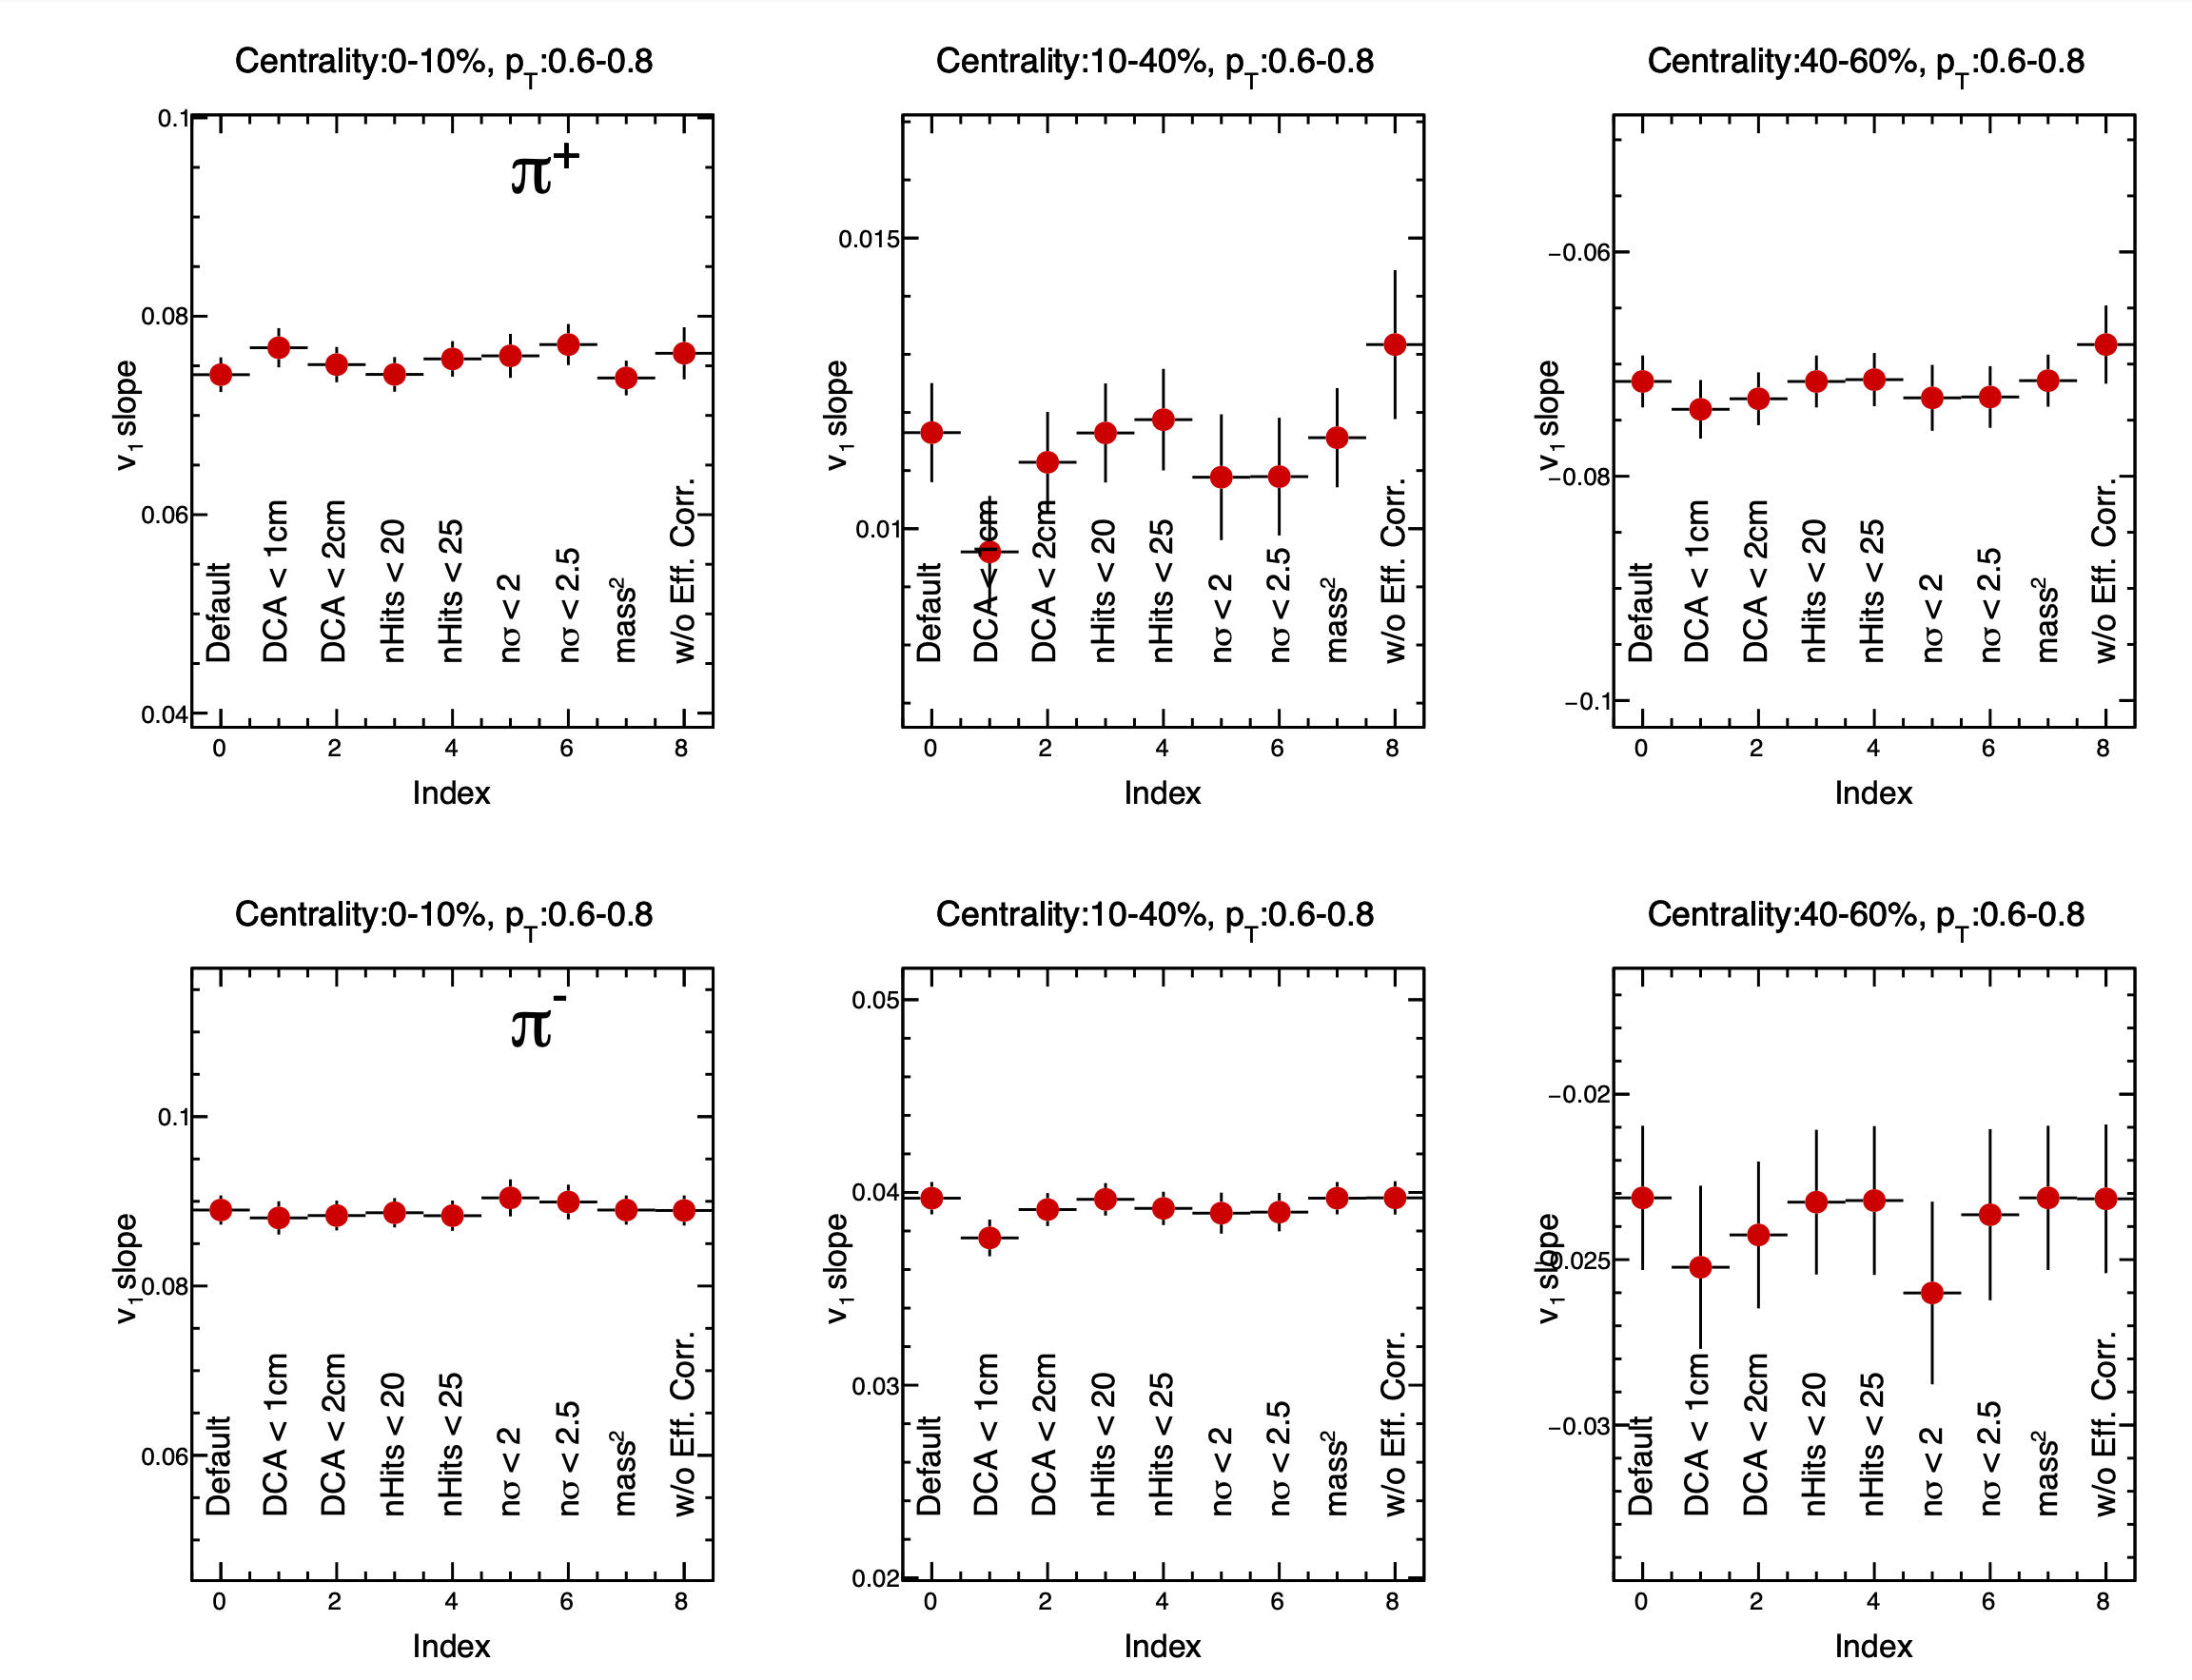
\includegraphics[width=0.85\linewidth]{figures/chapter03/3p5gev_pion_v1slopeIndex_sysUnc.png}
\caption{$v_1$ slope of pions as function of systematic sources at $\sqrt{s_{NN}}$ = 3.5 GeV.}
\label{fig:3p5gev_pion_v1slopeIndex_sysUnc}
\end{figure}

\begin{figure}[hbt!]
\centering
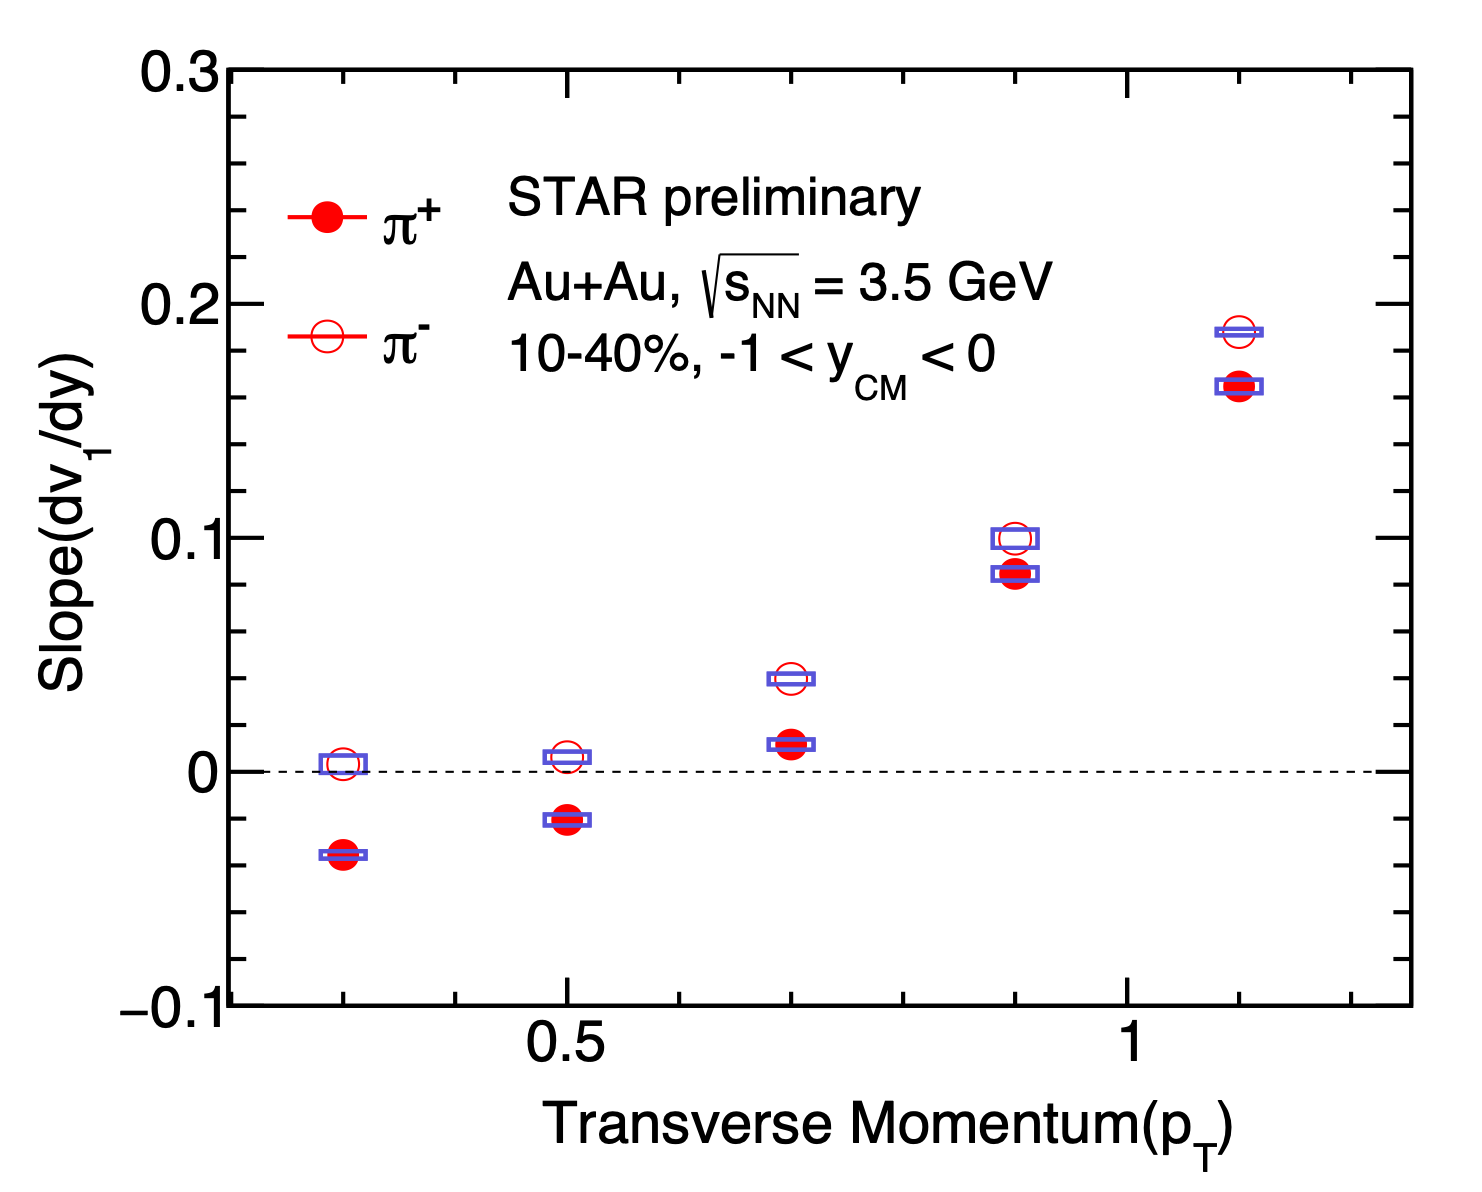
\includegraphics[width=0.55\linewidth]{figures/chapter03/3p5gev_pion_v1slopePt.png}
\caption{$v_1$ slope of pions as function of transverse momentum at $\sqrt{s_{NN}}$ = 3.5 GeV.}
\label{fig:3p5gev_pion_v1slopePt}
\end{figure}

\subsection{Directed flow of $K^{0}_{S}$, $\Lambda$}

Invariant mass method is applied to extract $v_1$ of $K^{0}_{S}$ and $\Lambda$. 
The ideal of this method is to seperate $v_1$ of signal from backgroud,  
where the $v_1$ of signal and backgroud could be expressed as equation~\ref{eq:invMass}.
Note that "Sig" denotes the signal yield, "Bg" denotes the backgroud yield, 
and $v_1$ of backgroud is taken as the second order polynomial function, 
$v_1^{Sig+Bg}$ is calculated by $v_1^{Sig+Bg} = <cos(\phi-\Psi_{EP})>/R_1$.
Then, $v_1^{Sig}$ in various rapidity bins could be extracted by fitting the invariant mass distribution,
which are shown by Fig.~\ref{fig:3p5gev_K0s_invMass}


\begin{equation}
v_1^{S i g+B g}\left(m_{i n v}\right)=\frac{S i g}{S i g+B g} v_1^{S i g}+\frac{B g}{S i g+B g} v_1^{B g}
\label{eq:invMass}
\end{equation}

\begin{figure}[hbt!]
\centering
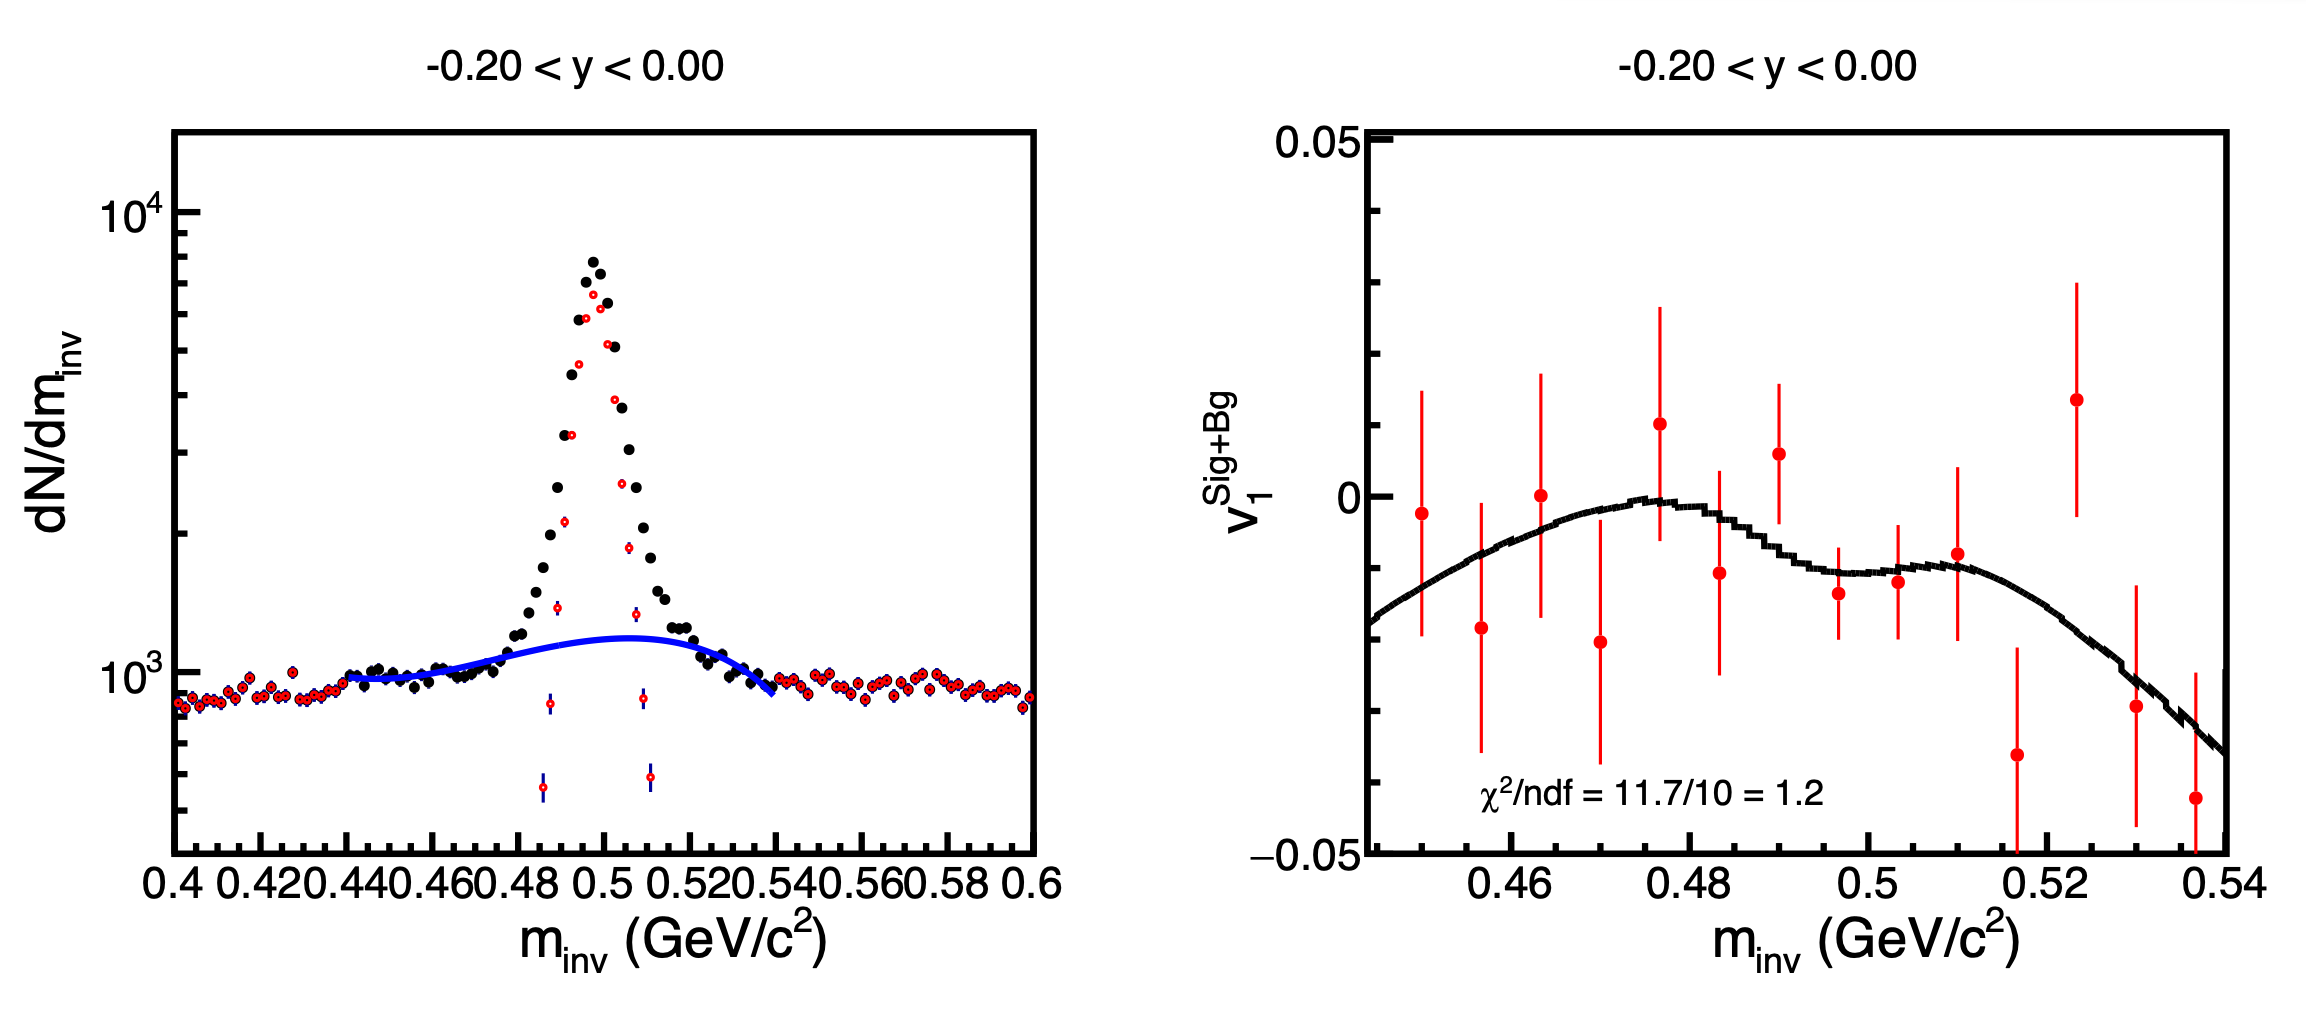
\includegraphics[width=0.85\linewidth]{figures/chapter03/3p5gev_K0s_invMass.png}
\caption{Invariant mass distribution of $K_S^0$ in 10-40\% centrality at $\sqrt{s_{NN}}$ = 3.5 GeV.}
\label{fig:3p5gev_K0s_invMass}
\end{figure}

\subsubsection{Rapidity dependence of $v_1$}

Fig.~\ref{fig:3p5gev_K0sLam_v1y} shows rapidity dependence of $K^0_S$ and $\Lambda$ $v_1$ within 10-40\% centrality at $\sqrt{s_{NN}}$ = 3.5 GeV,
where the $p_T$ cut are $0.4 < p_T < 1.6~GeV/c$, $0.4 < p_T < 2.0~GeV/c$ for $K^0_S$ and $\Lambda$, respectively. 

\begin{figure}[hbt!]
\centering
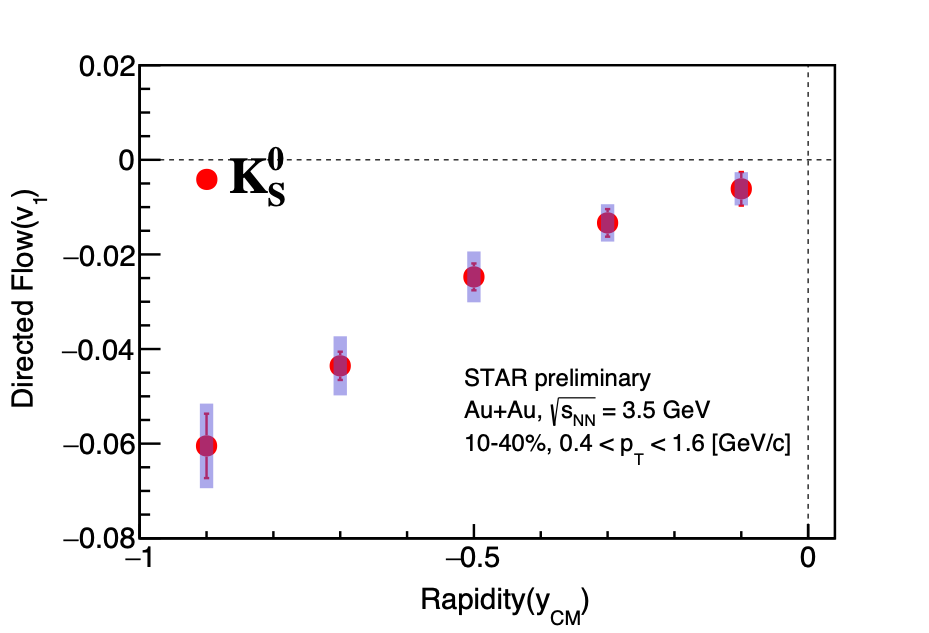
\includegraphics[width=0.45\linewidth]{figures/chapter03/3p5gev_K0s_v1VSy.png}
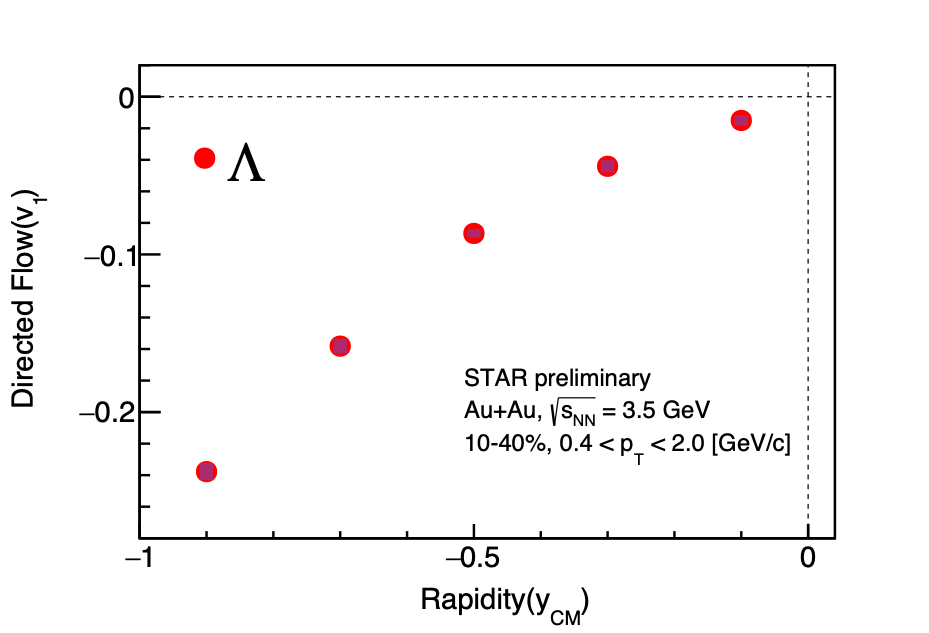
\includegraphics[width=0.45\linewidth]{figures/chapter03/3p5gev_Lambda_v1VSy.png}
\caption{$v_1$ of $K^0_S$ and $\Lambda$ as function of rapidity at $\sqrt{s_{NN}}$ = 3.5 GeV.}
\label{fig:3p5gev_K0sLam_v1y}
\end{figure}

\subsubsection{Transverse momentum dependence of $v_1(y)$}

Fig.~\ref{fig:3p5gev_K0sLam_v1y_pt_cent1} shows rapidity dependence of $K^0_S$ and $\Lambda$ $v_1$ within $p_T$ windows in 10-40\% centrality at $\sqrt{s_{NN}}$ = 3.5 GeV.
Note that the solid and dashed line in the plots are cubic function: $v_1(y) = a*y + b*y^3$. 
The coefficient of the linear term "a" is so called $v_1$ slope in the mid-rapidity($dv_1/dy|_{y=0}$).

\begin{figure}[hbt!]
\centering
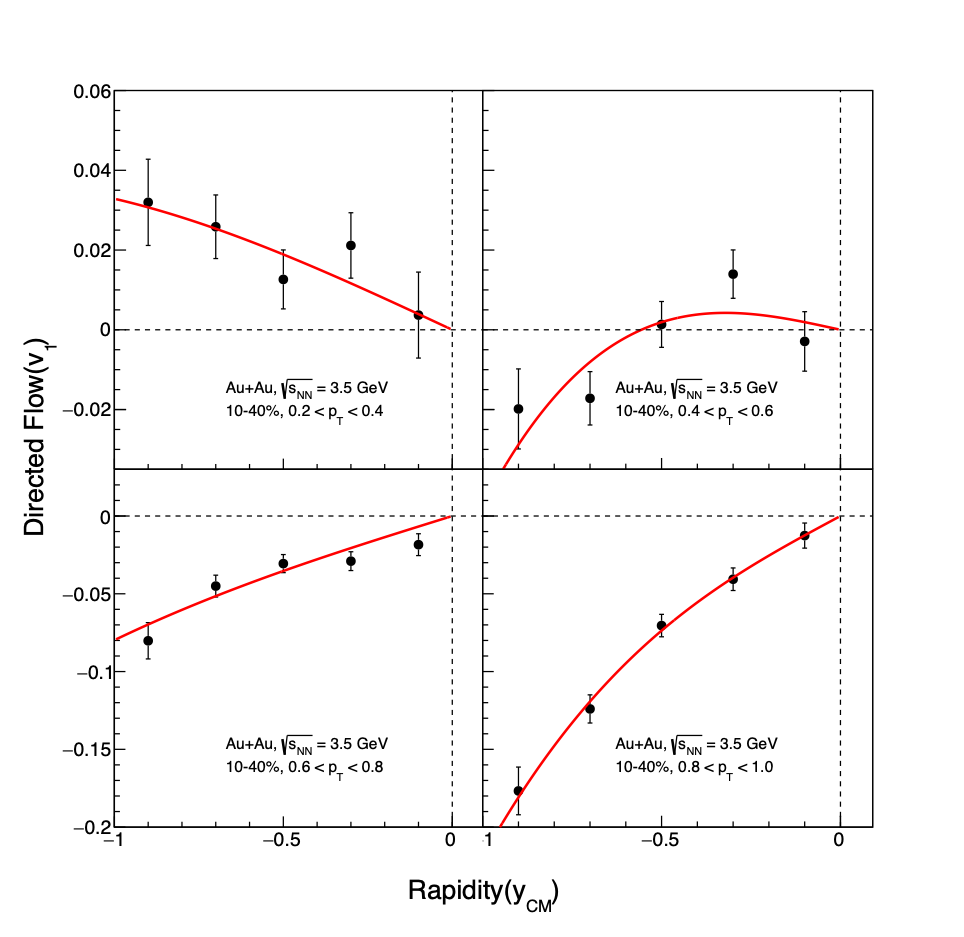
\includegraphics[width=0.45\linewidth]{figures/chapter03/3p5gev_K0s_v1VSy_pT_cent1.png}
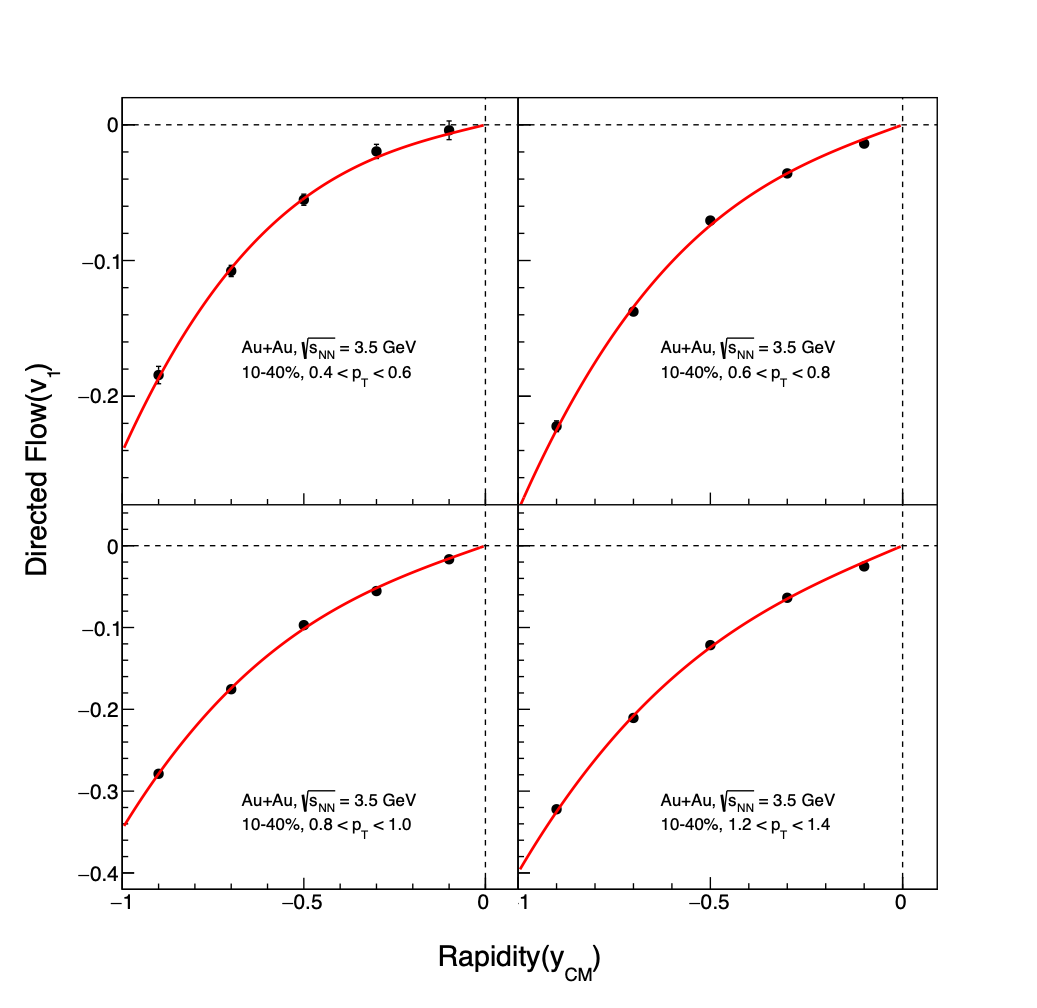
\includegraphics[width=0.45\linewidth]{figures/chapter03/3p5gev_Lambda_v1VSy_pT_cent1.png}
\caption{$v_1$ of $K^0_S$ (left) and $\Lambda$ (right) as function of rapidity within $p_T$ windows in 10-40\% centrality at $\sqrt{s_{NN}}$ = 3.5 GeV.}
\label{fig:3p5gev_K0sLam_v1y_pt_cent1}
\end{figure}

Fig.~\ref{fig:3p5gev_K0sLam_v1Slope_pt} show $p_T$ dependence of $v_1$ slope for $K^0_S$ and $\Lambda$, respectively.
$K^0_S$ show negative $v_1$ slopes at low $p_T$ ($p_T < 0.6$ GeV/$c$), which behaviors like charged kaons, 
while there is no anti-flow for $\Lambda$ at low $p_T$.

\begin{figure}[hbt!]
\centering
\includegraphics[width=0.45\linewidth]{figures/chapter03/3p5gev_K0s_v1Slope_pT.png}
\includegraphics[width=0.45\linewidth]{figures/chapter03/3p5gev_Lambda_v1Slope_pT.png}
\caption{$v_1$ slope of $K^0_S$ (left) and $\Lambda$ (right) as function of $p_T$ in 10-40\% centrality at $\sqrt{s_{NN}}$ = 3.5 GeV.}
\label{fig:3p5gev_K0sLam_v1Slope_pt}
\end{figure}

\subsubsection{Systematic uncertainty}

For systematic uncertainty estimate of $K^0_S$ and $\Lambda$ $v_1$, 
which are reconstructed by KF particle package, 
we take track quality cut (nHitsFit), PID cuts (n$\sigma_{particle}$ and $\chi^2_{prim}$ of daughters), and resolution as systematic uncertainty sources.
TABLE~\ref{tab:lamK0s_sysUnc} show the systematic uncertainty sources chosen for directed measurement of $\pi$, K, p.
We assume that these sources are uncorrelated. According to Barlow Test~\cite{barlow2002systematic}, the differences between the default source and the variation are required
to be smaller than the one of their statistical uncertainties, otherwise it would not be taken as systematic uncertainty since the statistical fluctuation dominants.
At last, the maximum deviation from the default value was chosen as the systematic uncertainty. 
The total systematic uncertainties could be obtained by adding uncertainties brought from each sources in quadrature, 
which could be expressed as the equation~\ref{eq:sysUnc_lamK0s}.

\begin{table}
    \centering
    \begin{tabular}{|c|c|c|c|} \hline  
         Cuts&  Default&  var1& var2\\ \hline  
         nHitsFit($>$)&  15&  20& 25\\
 $\chi^2_{prim}$& 10& 5&15\\\hline  
         n$\sigma_{particle}$&  3&  2& 2.5\\ \hline 
         $R_{11}$&  EPD-C'&  EPD-D& \\ \hline 
    \end{tabular}
    \caption{Systematic uncertainty sources for $K^0_S$ and $\Lambda$, Note that EPD-C' is EPD-AB vs. EPD-C' and TPC-B, and EPD-D is EPD-AB vs. EPD-D and TPC-B,
    which are shown in the Fig.~\ref{fig:1st_resolution}}
    \label{tab:lamK0s_sysUnc}
\end{table}



\begin{equation}
s y s. Unc_{\text {total }}=\sqrt{\left(y_{n H i tsFit}-y_{d e f}\right)^2+\left(y_{\chi^2_{prim}}-y_{d e f}\right)^2+\left(y_{n \sigma}-y_{d e f}\right)^2+\left(y_{Res}-y_{d e f}\right)^2}
\label{eq:sysUnc_lamK0s}
\end{equation}

Fig.~\ref{fig:3p5gev_K0s_v1y_sysUnc} and Fig.~\ref{fig:3p5gev_lam_v1y_sysUnc} 
illustrate the rapidity dependence of $v_1$ from various systematic sources at $\sqrt{s_{NN}}$ = 3.5 GeV for $K^0_S$ and $\Lambda$, respectively.
Fig.~\ref{fig:3p5gev_K0s_v1yPt_sysUnc} and Fig.~\ref{fig:3p5gev_lam_v1yPt_sysUnc} show $v_1(y)$ within narrow $p_T$ windows of $K^0_S$ and $\Lambda$, respectively. 
The $v_1$ slopes extracted in the mid-rapidity are summarized with Fig.~\ref{fig:3p5gev_K0s_v1slopeIndex_sysUnc} and Fig.~\ref{fig:3p5gev_lam_v1slopeIndex_sysUnc}.


\begin{figure}[hbt!]
\centering
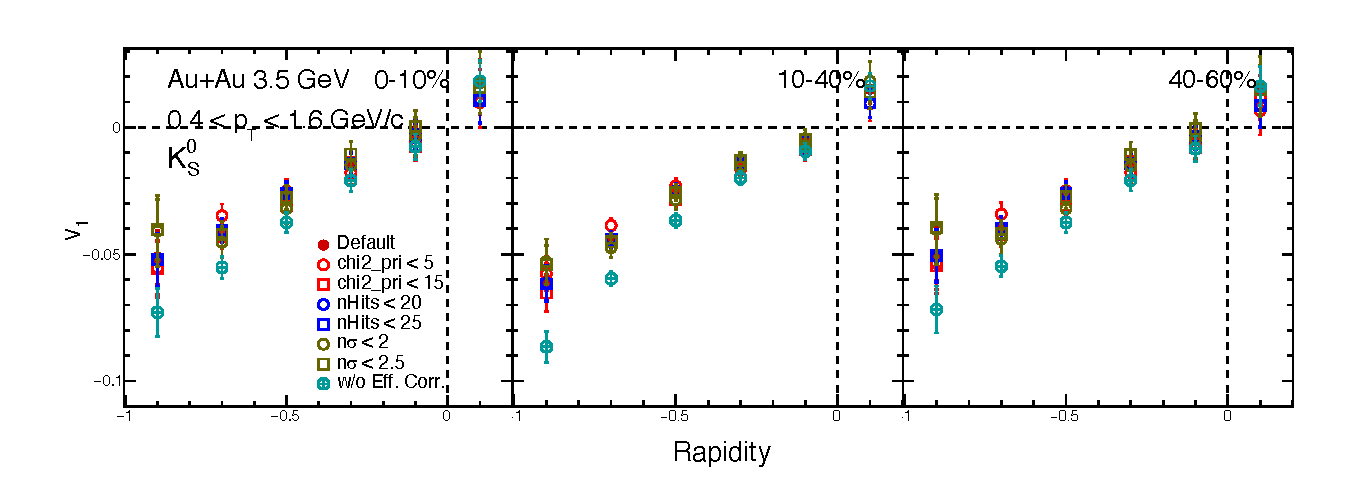
\includegraphics[width=0.95\linewidth]{figures/chapter03/3p5gev_K0s_v1y_sysUnc.pdf}
\caption{$v_1$ of $K^0_S$ as function of rapidity from systematic sources at $\sqrt{s_{NN}}$ = 3.5 GeV.}
\label{fig:3p5gev_K0s_v1y_sysUnc}
\end{figure}

\begin{figure}[hbt!]
\centering
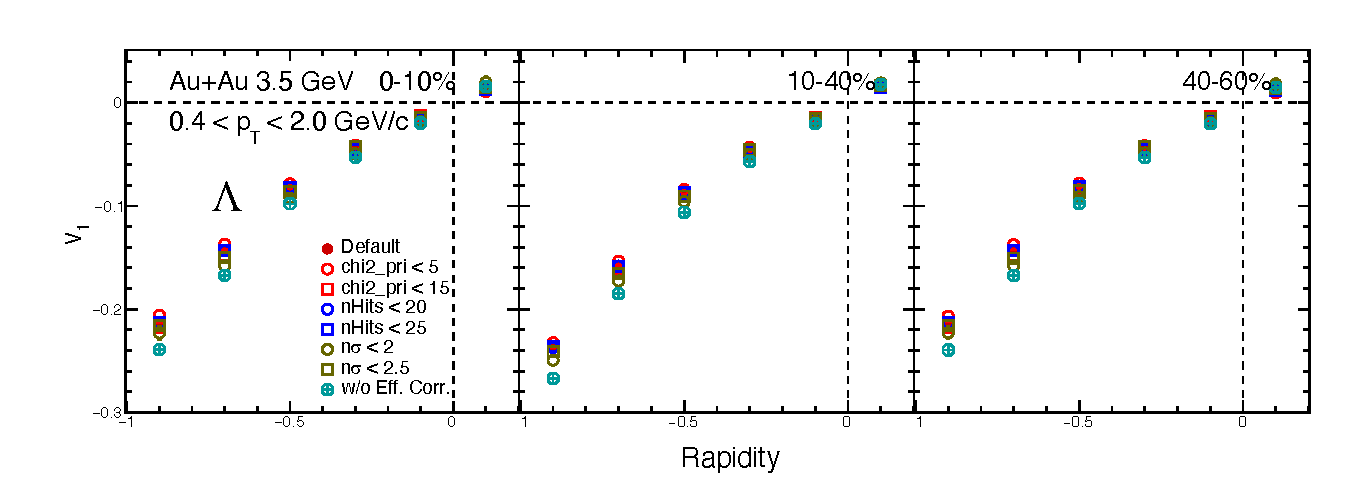
\includegraphics[width=0.95\linewidth]{figures/chapter03/3p5gev_lam_v1y_sysUnc.pdf}
\caption{$v_1$ of $\Lambda$ as function of rapidity from systematic sources at $\sqrt{s_{NN}}$ = 3.5 GeV.}
\label{fig:3p5gev_lam_v1y_sysUnc}
\end{figure}


\begin{figure}[hbt!]
\centering
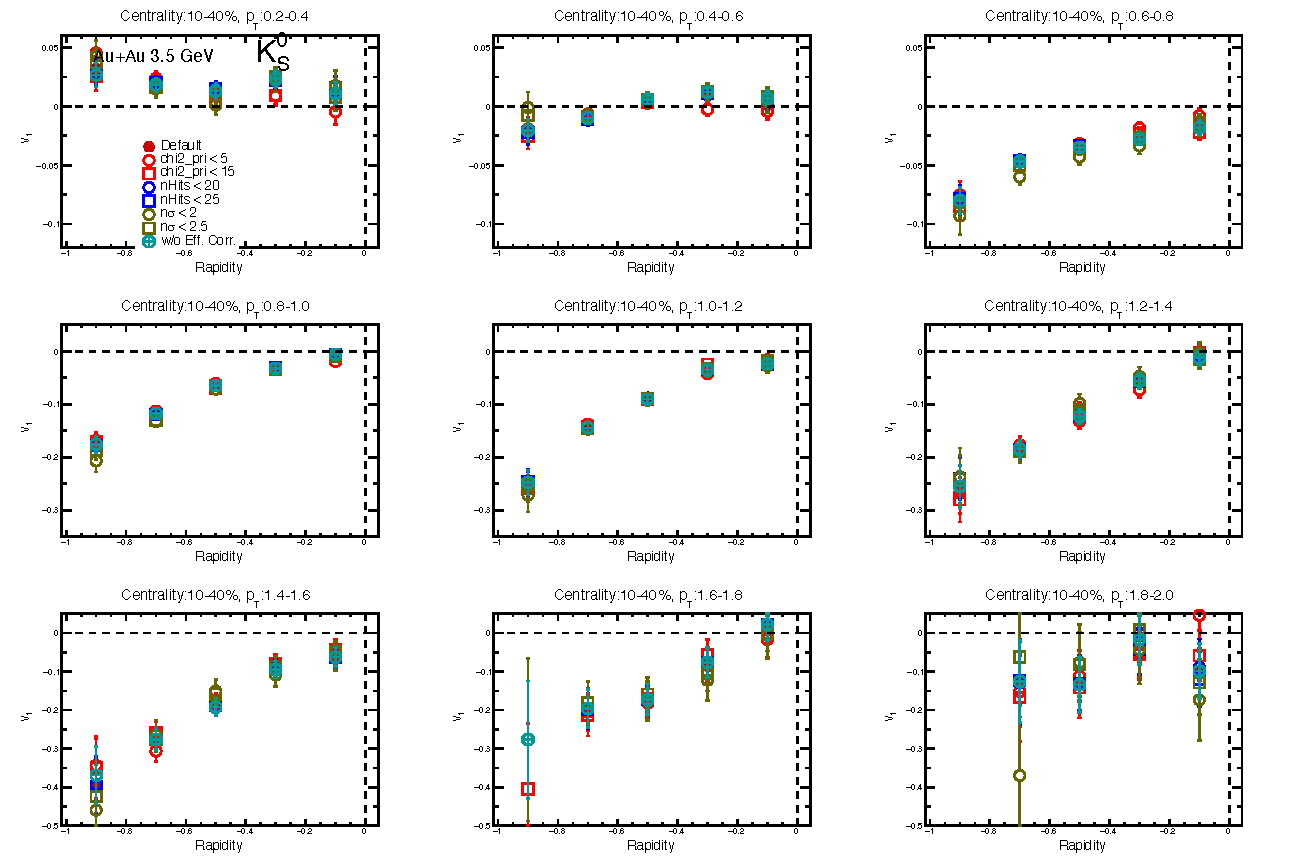
\includegraphics[width=0.95\linewidth]{figures/chapter03/3p5gev_K0s_v1yPt_sysUnc.pdf}
\caption{$v_1$ of $K^0_S$ as function of rapidity within $p_T$ windows at $\sqrt{s_{NN}}$ = 3.5 GeV.}
\label{fig:3p5gev_K0s_v1yPt_sysUnc}
\end{figure}

\begin{figure}[hbt!]
\centering
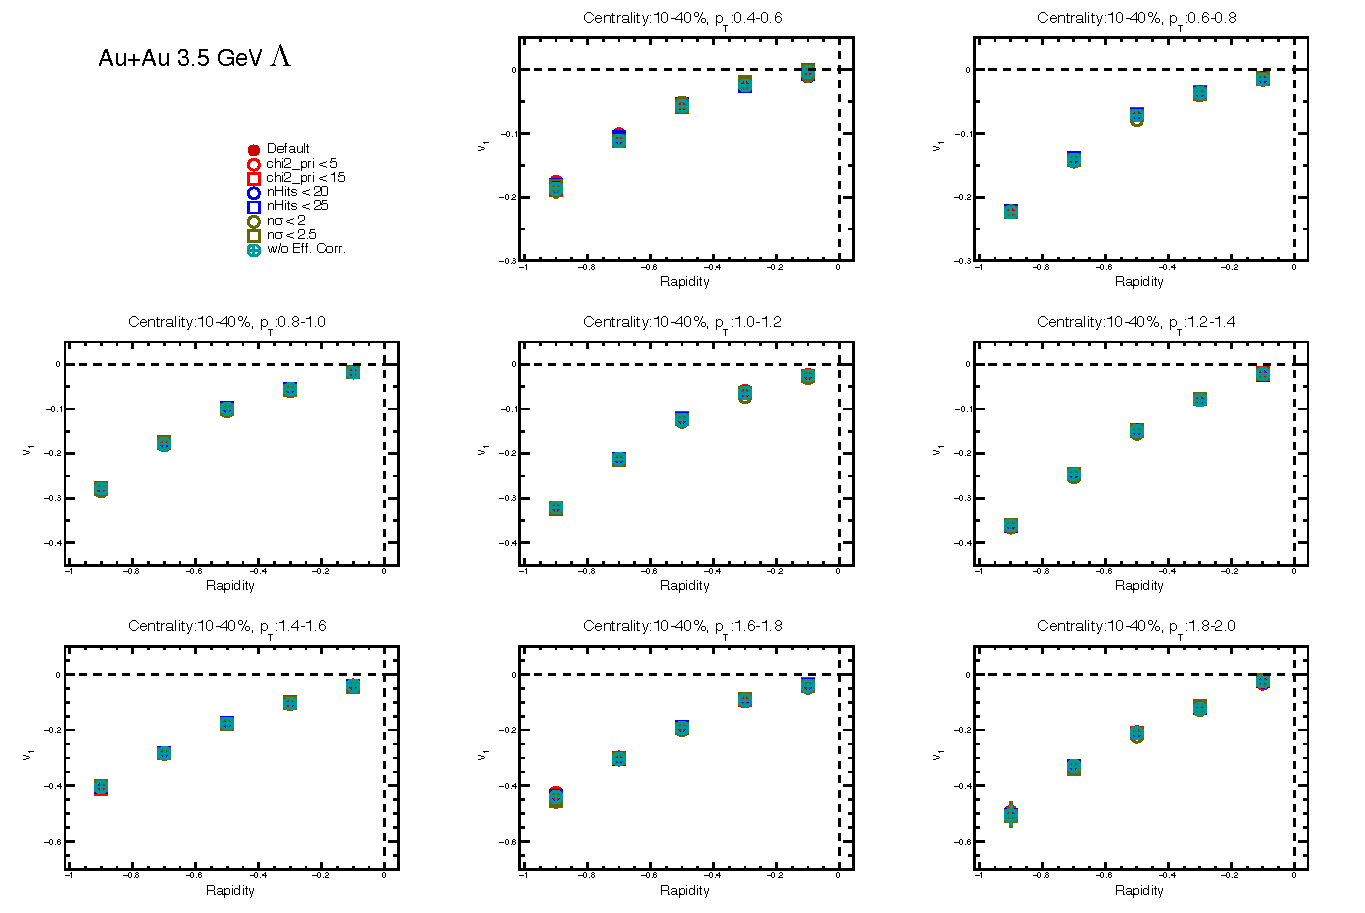
\includegraphics[width=0.95\linewidth]{figures/chapter03/3p5gev_lam_v1yPt_sysUnc.pdf}
\caption{$v_1$ of $\Lambda$ as function of rapidity within $p_T$ windows at $\sqrt{s_{NN}}$ = 3.5 GeV.}
\label{fig:3p5gev_lam_v1yPt_sysUnc}
\end{figure}

\begin{figure}[hbt!]
\centering
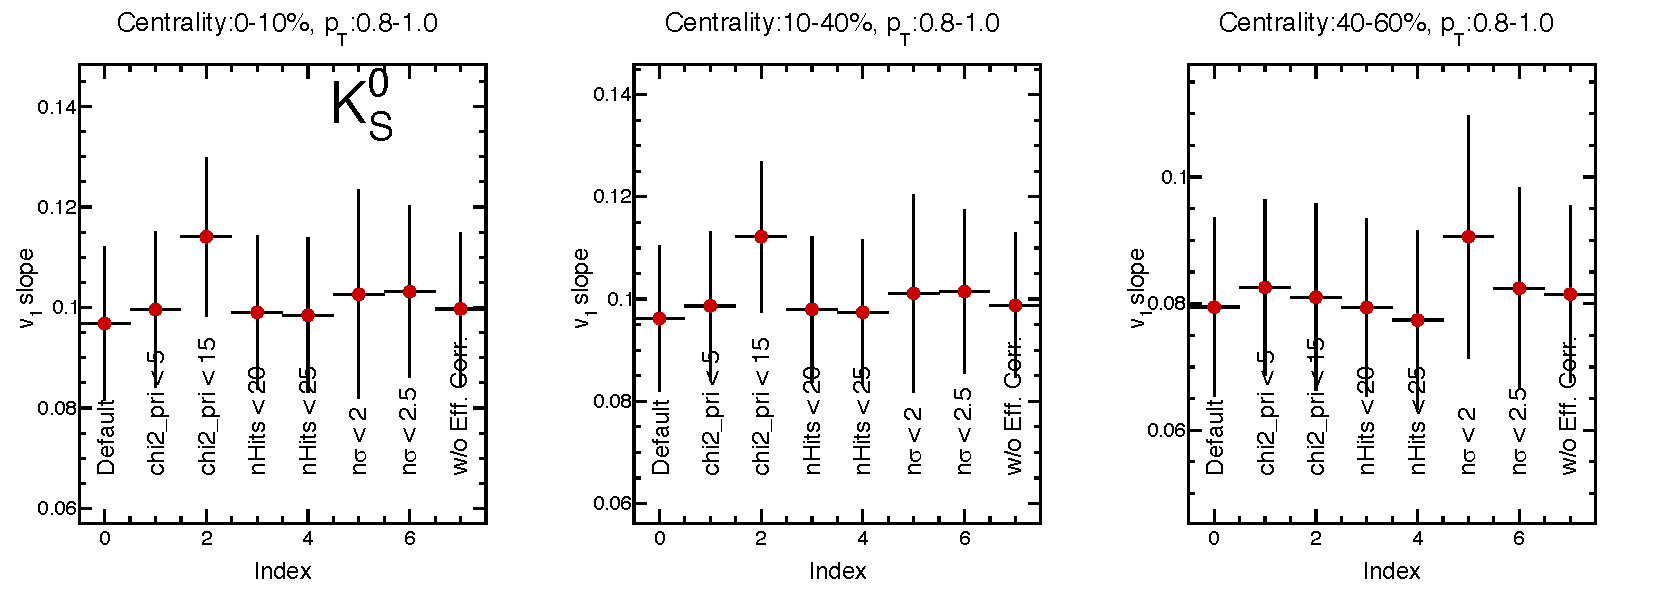
\includegraphics[width=0.85\linewidth]{figures/chapter03/3p5gev_K0s_v1slopeIndex_sysUnc.pdf}
\caption{$v_1$ slope of $K^0_S$ as function of systematic sources at $\sqrt{s_{NN}}$ = 3.5 GeV.}
\label{fig:3p5gev_K0s_v1slopeIndex_sysUnc}
\end{figure}

\begin{figure}[hbt!]
\centering
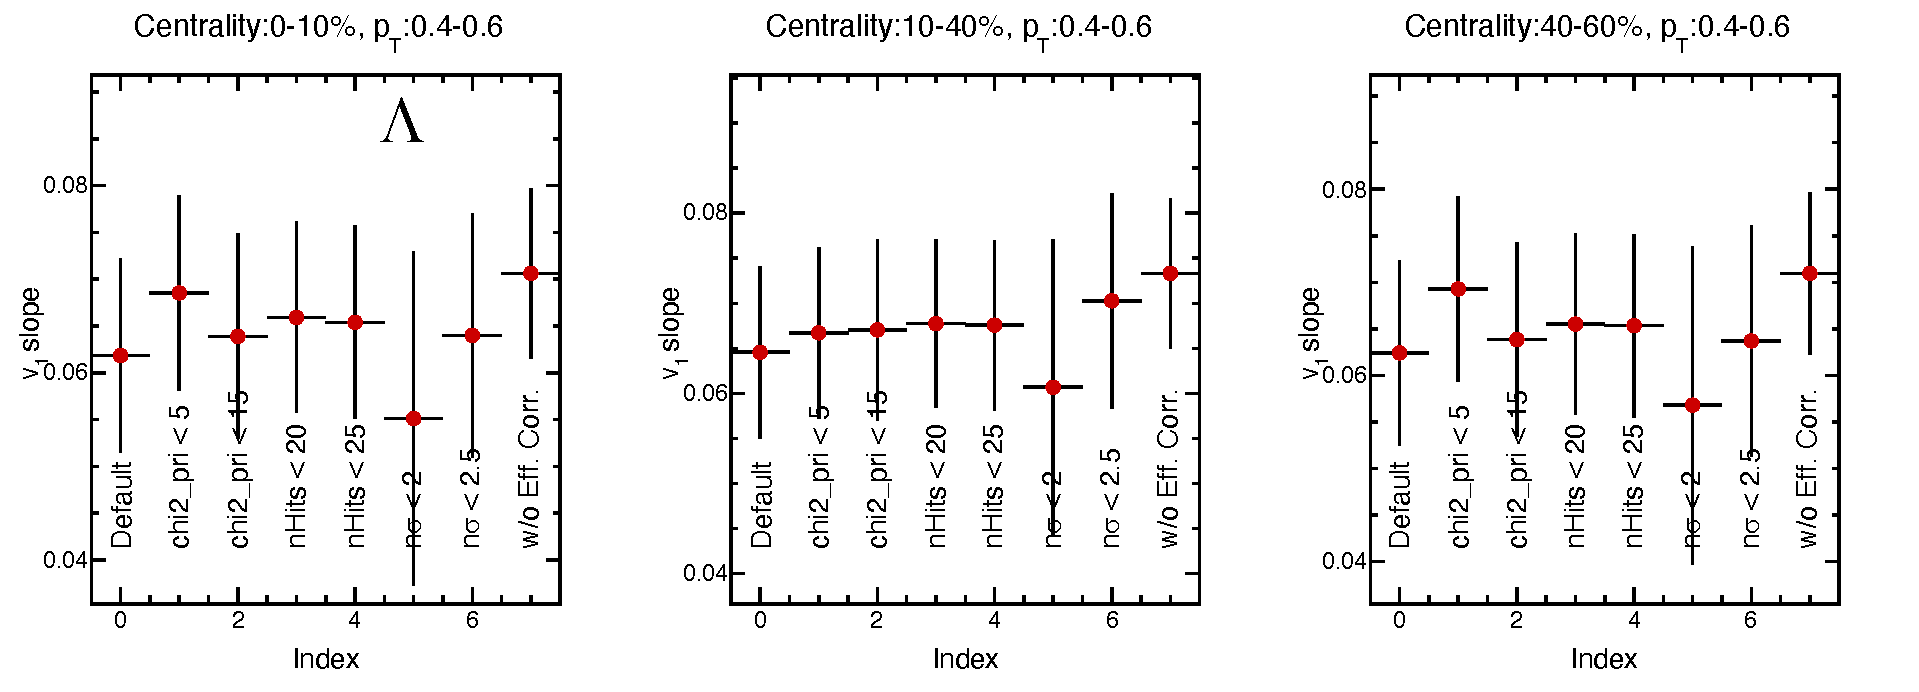
\includegraphics[width=0.85\linewidth]{figures/chapter03/3p5gev_lam_v1slopeIndex_sysUnc.pdf}
\caption{$v_1$ slope of $\Lambda$ as function of systematic sources at $\sqrt{s_{NN}}$ = 3.5 GeV.}
\label{fig:3p5gev_lam_v1slopeIndex_sysUnc}
\end{figure}
\section{Summary}

We present directed flow measurement for $\pi^{\pm}, K^{\pm}, p$ and $K^0_S, \Lambda$
in Au + Au collisions at $\sqrt{s_{NN}}$ = 3.0, 3.2, 3.5, and 3.9 GeV.
The $p_T$ dependence of $v_1$ slope in the mid-rapidity shows
that there is anti-flow at low $p_T$ ($p_T <$ 0.6 GeV/$c$ ) for $\pi^{+}$ and kaons ($K^{\pm}, K^0_S$) in the mid-central 10 - 40\% collisions.
By contrast, the baryons (proton and lambda) don't show anti-flow low $p_T$.
Moreover, the centrality dependence of $dv_1/dy$ shows
that more negative $v_1$ slope could be observed in the more peripheral collisions.
It indicates that the anti-flow might be related with spectator shadowing effect.
At last, the JAM model calculation can reproduce anti-flow at low $p_T$ without incorporating kaon potential.
With the data measurement and model calculation,
we conclude that the spectator shadowing effect can lead to anti-flow of kaons, no need of the earlier claimed kaon potential.


\clearpage

\newpage

% 其他部分
% 附录
\appendix
% !TeX root = ../analysisnote.tex

\section{appendix}

\clearpage


\newpage

% 参考文献
\bibliography{ref/refs}

\clearpage


\end{document}
